%%%%%%%%%%%%%%%%%%%% book.tex %%%%%%%%%%%%%%%%%%%%%%%%%%%%%
%
% sample root file for the chapters of your "monograph"
%
% Use this file as a template for your own input.
%
%%%%%%%%%%%%%%%% Springer-Verlag %%%%%%%%%%%%%%%%%%%%%%%%%%


% RECOMMENDED %%%%%%%%%%%%%%%%%%%%%%%%%%%%%%%%%%%%%%%%%%%%%%%%%%%
\documentclass[envcountsame,envcountchap]{svmono}
%\documentclass[envcountsame,envcountchap]{svmono}

% choose options for [] as required from the list
% in the Reference Guide, Sect. 2.2

\usepackage{makeidx}         % allows index generation
\usepackage{graphicx}        % standard LaTeX graphics tool
\usepackage{amsmath,amssymb}         % matrices
\usepackage{enumerate}
\usepackage{dynkin-diagrams}
\usepackage{pstricks}
\usepackage{pdfpages}
\usepackage{svg}
\usepackage{pst-all}
\usepackage{pstricks-add}
\usepackage{pgfplots}
\usetikzlibrary{arrows}

                             % when including figure files
\usepackage{multicol}        % used for the two-column index
\usepackage[bottom]{footmisc}% places footnotes at page bottom
% etc.
% see the list of further useful packages
% in the Reference Guide, Sects. 2.3, 3.1-3.3


\DeclareMathOperator{\End}{End}
\DeclareMathOperator{\Aut}{Aut}
\DeclareMathOperator{\Hom}{Hom}
\DeclareMathOperator{\support}{supp}


% NEW COMMANDS

%It is standard in Latex to write "macros" which are shorthand for an entire series of instructions. Here are some examples

%Number sets
\newcommand{\N}{\mathbb N}
%So typing \N produces the correct mathematical symbol for the natural numbers
\newcommand{\Z}{\mathbb Z}
\newcommand{\Q}{\mathbb Q}
\newcommand{\R}{\mathbb R}
\newcommand{\C}{\mathbb C}
\newcommand{\K}{\mathbb K}
%notations quelquonques
\newcommand{\tg}[1]{\textbf{#1}}
\newcommand{\ub}[1]{\overline{#1}}

%notations des objets simples
\newcommand{\es}{\emptyset}
\newcommand{\nes}{$\not= \emptyset$}
\newcommand{\sub}{\subset}
\newcommand{\norm}[2]{\lVert #1 \lVert_{#2}}
\newcommand{\vect}[2]{(#1_1,#1_2, \dots, #1_#2)}
\newcommand{\modu}[1]{\lvert#1\lvert}
\newcommand{\B}[3]{B_{#1}\big(#2,#3\big[}
%notations mathématiques
\newcommand{\lb}{\lbrack}
\newcommand{\rb}{\rbrack}
\newcommand{\lv}{\lVert}
%limits and sum
\newcommand{\s}[2]{\sum\limits_{#1}^{#2}}
\newcommand{\li}[2]{\xrightarrow[#1\rightarrow#2]{}}
\newcommand{\lis}[1]{\xrightarrow[n\rightarrow+\infty]{#1}}
\newcommand{\lif}[1]{\xrightharpoonup[n\rightarrow+\infty]{#1}}
\newcommand{\lic}[3]{\xrightarrow[#1\rightarrow#2]{#3}}

\newcommand{\bcup}[2]{\bigcup\limits_{#1}^{#2}}
\newcommand{\bcap}[2]{\bigcap\limits_{#1}^{#2}}

\newcommand{\inv}[1]{\frac{1}{#1}}
\newcommand{\prods}[2]{\langle\qq #1\qq,\qq#2\qq\rangle}

\newcommand{\restr}[2]{#1_{\mkern 2mu \vrule height 2ex\mkern2mu #2} }
\newcommand{\quot}[2]{{\raisebox{.2em}{$#1$}\left/\raisebox{-.2em}{$#2$}\right.}}
\newcommand{\limite}[2]{\underset{#1\rightarrow#2}{\text{lim}}}
\newcommand{\espp}[2]{Ker\big(u-{#1} Id_{#2}\big)}
\newcommand{\fct}[4]{\qq:\qq #1\qq\longrightarrow\qq #2\qq :\qq #3\qq \mapsto\qq #4}

\newcommand{\lam}{\lambda}
\newcommand{\q}{\quad}
\newcommand{\qq}{\text{ }}

\newcommand{\liste}[2]{#1_1, #1_2,..,#1_{#2}}

\newcommand{\maxx}[1]{\underset{#1}{\text{max}}}
\newcommand{\minn}[1]{\underset{#1}{\text{min}}}
\newcommand{\supp}[1]{\underset{#1}{\text{sup}}}
\newcommand{\inff}[1]{\underset{#1}{\text{inf}}}

\newcommand{\fctt}[2]{\qq:\qq#1\qq\rightarrow\qq#2}
\newcommand{\liminff}[1]{\underset{#1\rightarrow+\infty}{\text{liminf}}}
\newcommand{\limsupp}[1]{\underset{#1\rightarrow+\infty}{\text{limsup}}}

\newcommand{\adh}[2]{\text{Adh}_{#1}\big(#2\big)}
\newcommand{\wed}[3]{#1_#2\wedge\dots \wedge #1_#3}


\makeindex             % used for the subject index
                       % please use the style svind.ist with
                       % your makeindex program


%%%%%%%%%%%%%%%%%%%%%%%%%%%%%%%%%%%%%%%%%%%%%%%%%%%%%%%%%%%%%%%%%%%%%

\begin{document}

\author{MATH-F-427 students}
\title{Coxeter groups}
\subtitle{Course notes}
\maketitle

\frontmatter%%%%%%%%%%%%%%%%%%%%%%%%%%%%%%%%%%%%%%%%%%%%%%%%%%%%%%

\tableofcontents


\mainmatter%%%%%%%%%%%%%%%%%%%%%%%%%%%%%%%%%%%%%%%%%%%%%%%%%%%%%%%
\part{Coxeter groups}
\chapter{Preliminaries}

This chapter is based on the first chapter of \cite{magnusCombinatorialGroupTheory2004}. This constitutes a recap of what groups are and how they are generated.\\

We recall that a group $(G,\cdot)$ is a non-empty set $G$ of elements equipped with a binary operation $\cdot\qq :\qq  G \times G \rightarrow G$ for which the next properties are satisfied :

\begin{itemize}
  \item \textbf{Associativity:} The operation $\cdot$ is associative, which means that for any elements $a,b,c \in G$ :
    $$(ab)c = a(bc)$$

  \item \textbf{Identity element:} There exists an element of $G$ noted $e$ for which :

  $$a\cdot e = e\cdot a = a$$

  \item \textbf{Inverse element:} For any $a \in G$ there exists an \textit{element} $a^{-1}$ for which :
  $$ a\cdot a^{-1} = a^{-1} \cdot a = e $$
\end{itemize}

There are a lot of ways to define groups. However, the two most ``common" ways in the everyday mathematics is to consider set of \textit{symmetries} or to give an explicit presentation of the group in terms of generators and relations.

\section{Symmetric groups}

\begin{definition}[Symmetric group]
The symmetric group on the set $M$ is the group whose elements are permutations of the elements of $M$ and its operation is the permutation composition. If $M = \{1,\dots, n \}$ we call it $S_n$. \cite{saganSymmetricGroup2001}.
\end{definition}

\begin{proposition}$S_n$ has order $n!$ and every group $G$ of order $n$ is a subgroup of $S_n$.
\end{proposition}

%\subsection{Permutations}

Symmetric groups are based on the behave of permutations and as we explain, there are a very important example of groups since every group is a subgroup of such. The purpose of this subsection is to define the operation on permutations.


\begin{definition}[Two-line notation]
Given a permutation function $\pi$ of ${1,...,n}$, we represent it by listing every elements of the set ${0,...,n}$ in two lines, where the first line represent the starting elements, and the second one, their images through the function $\pi$ :

\begin{equation}
  \begin{pmatrix}
   1 & 2 & 3 & 4 & 5 & \dots & n \\
   \pi(1) & \pi(2) & \pi(3) & \pi(4) & \pi(5) & \ & \pi(n)
 \end{pmatrix}
\end{equation}

\end{definition}


\begin{definition}[Cycle notation]Given $i \in \{1,\dots,n\}$ and $\pi$ a permutation function of $\{1,\dots,n\}$, the elements of the sequence $i, \pi(i), \pi^2(i),\dots$ cannot all be distinct due to the pigeon hole principle. In particular, there must exists a power $p \in \mathbb{N}$ such that $\pi^p(i) = i$. This allow us to write the permutation as a product of cycles of the type :

\begin{equation}
  (i, \pi(i), \pi^2(i), \dots, \pi^{p-1}(i))
\end{equation}
\end{definition}

This means that, given a cycle $(i,j,k)$, the element $i$ is sent to $j$, $j$ is sent to $k$ and $k$ is sent to $i$, cyclically, e.g. the permutation $23145$ of $ \{1,2,3,4,5\}$ can be written with cycle notation as $(1,2,3)(4)(5)$. Remark that every element of the set has to be used.

\section{Presentation of groups}
\label{sec:pres_group}

In this section we show how a group can be defined by generators and relations :

\begin{definition}
  A group can be defined by:
  \begin{equation}
    Gr \cong \langle G | R\rangle
  \end{equation}
where $G = \{a,b,c,\dots\}$ is the set of \emph{generators} and $R = \{A,B,C,\dots\}$ is the set of \emph{relations} such that every $X \in R$ is a word in $(G\cup G^{-1})^*$ satisfying $X = 1$.
\end{definition}

\begin{example}
The dihedral group $D_n$ can be presented in the following way; where $q$ is a rotation and $r$ a reflection :

$$D_n \cong \langle \{q,r\} | \{r^2, q^n, rqrq\} \rangle$$
\end{example}


\chapter{Coxeter groups}

\section{Motivations}
Let us explain the interest and motivation of Coxeter groups by analysing the symmetric group $S_3$, which is a standard example of Coxeter group. This group can be defined in three ways.

\begin{figure}
  \begin {center}
  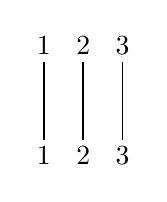
\begin{tikzpicture}
  	% general shift to north east
    \draw (0,1+0.2) node {$1$};
    \draw (0.5,1+0.2) node {$2$};
    \draw (1,1+0.2) node {$3$};
  	\draw[semithick] (0,0) -- (0,1);% first line
  	\draw[semithick] (0.5,0) -- (0.5,1);% second line
  	\draw[semithick] (1,0) -- (1,1);% third line
    \draw (0,-0.2) node {$1$};
    \draw (0.5,-0.2) node {$2$};
    \draw (1,-0.2) node {$3$};
  \end{tikzpicture}

  \caption{The wiring diagram for the permutation $123$.}
  \end{center}
\label{fig:wiring}
\end{figure}

\begin{figure}
  \begin {center}
  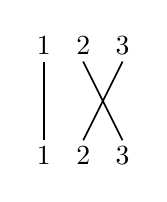
\begin{tikzpicture}
    % general shift to north east
    \draw (0,1+0.2) node {$1$};
    \draw (0.5,1+0.2) node {$2$};
    \draw (1,1+0.2) node {$3$};
    \draw[semithick] (0,0) -- (0,1);% first line
    \draw[semithick] (0.5,0) -- (1,1);% second line
    \draw[semithick] (1,0) -- (0.5,1);% third line
    \draw (0,-0.2) node {$1$};
    \draw (0.5,-0.2) node {$2$};
    \draw (1,-0.2) node {$3$};
  \end{tikzpicture}
  \caption{The wiring diagram for the permutation $132$.}
  \end{center}
\label{fig:wiring_23}
\end{figure}

\begin{figure}
  \begin {center}
  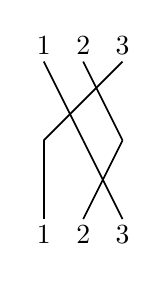
\begin{tikzpicture}
    % general shift to north east
    \draw (0,2+0.2) node {$1$};
    \draw (0.5,2+0.2) node {$2$};
    \draw (1,2+0.2) node {$3$};
    \draw[semithick] (0,0) -- (0,1);% first line
    \draw[semithick] (0,1) -- (1,2);% first line
    \draw[semithick] (0.5,0) -- (1,1);% second line
    \draw[semithick] (0.5,1) -- (0,2);% second line
    \draw[semithick] (1,0) -- (0.5,1);% third line
    \draw[semithick] (1,1) -- (0.5,2);% third line
    \draw (0,-0.2) node {$1$};
    \draw (0.5,-0.2) node {$2$};
    \draw (1,-0.2) node {$3$};
  \end{tikzpicture}

  \caption{The wiring diagram for the permutation composition $132 \circ 231$.}
  \end{center}
\label{fig:wiring_compo}
\end{figure}


\begin{figure}
  \begin{center}
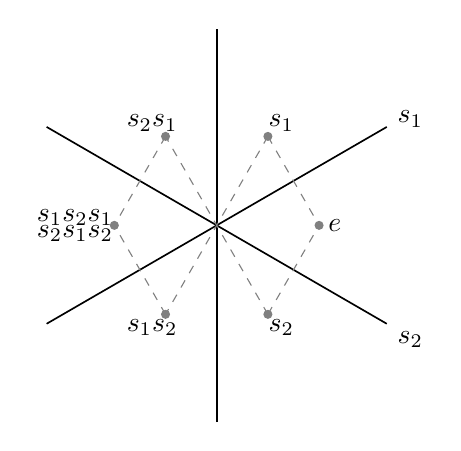
\begin{tikzpicture}
	% general shift to north east
	\draw[semithick] (0,-2.5) -- (0,2.5);% center line
  \draw[semithick] (-2.16,1.25) -- (2.16,-1.25);% first symmetry
  \draw[semithick] (2.16,1.25) -- (-2.16,-1.25);% second symmetry

  \def\offX{0.65}
  \def\offY{1.13}
	\draw[dashed,color=gray] (0+\offX,0+\offY) -- (0.65+\offX,-1.13+\offY);% e to s_1
  \draw[dashed,color=gray] (0+\offX,0-\offY) -- (0.65+\offX,-1.13+\offY);% e to s_2
	\draw[dashed,color=gray] (0+\offX,0+\offY) -- (0-\offX,0-\offY);% s_1 to s_1s_2
  \draw[dashed,color=gray] (0+\offX,0-\offY) -- (0-\offX,0+\offY);% s_2 to s_2s_1
  \draw[dashed,color=gray] (0-\offX,0+\offY) -- (-1.3,0);% s_1s_2 to s_1s_2s_1
  \draw[dashed,color=gray] (0-\offX,0-\offY) -- (-1.3,0);% s_2s_1 to s_2s_1s_2

  \draw [fill=gray, color=gray](1.3,0) circle (0.05);
  \draw [fill=gray, color=gray](-1.3,0) circle (0.05);
  \draw [fill=gray, color=gray](0+\offX,0+\offY) circle (0.05);
  \draw [fill=gray, color=gray](0-\offX,0+\offY) circle (0.05);
  \draw [fill=gray, color=gray](0+\offX,0-\offY) circle (0.05);
  \draw [fill=gray, color=gray](0-\offX,0-\offY) circle (0.05); % s_1s_2

  % axis
  \def\offAx{0.2}
  \draw (2.16+\offAx+0.1,-1.25-\offAx) node {$s_2$};
  \draw (2.16+\offAx+0.1,+1.25+\offAx-0.1) node {$s_1$};

  \draw (1.5,0) node {$e$};
  \draw (-1.8,0+0.1) node {$s_1s_2s_1$};
  \draw (-1.8,0-0.1) node {$s_2s_1s_2$};
  \draw (0+\offX + 0.17,0+\offY + 0.17) node {$s_1$};
  \draw (0+\offX + 0.17,0-\offY - 0.17) node {$s_2$};
  \draw (0-\offX - 0.17,0+\offY + 0.17) node {$s_2s_1$};
  \draw (0-\offX - 0.17,0-\offY - 0.17) node {$s_1s_2$};
\end{tikzpicture}
\end{center}
\caption{Geometrical representation of $S_3$. The grey dotted lines represent the reflection applied between two points.}
\label{fig:geoS3}
\end{figure}

\begin{itemize}
  \item Combinatorially : Given a cyclic permutation, we can represent it as a \emph{wiring diagram}. Some examples of permutations of $123$ are given in the wire diagrams \ref{fig:wiring} and \ref{fig:wiring_23}. Their composition is given by the wire diagram \ref{fig:wiring_compo}.




  \item Algebraically : Presentation of groups as seen in section \ref{sec:pres_group}.
  \begin{equation}\label{equation donnant la form explicite de pi}
  \begin{split}
  S_3 \cong \langle \{s_1, s_2\} | \{ s_1s_2s_1 &= s_2s_1s_2 , s_1^2 = e, s_2^2 = e,\\
   &(s_1s_2)^3 = s_1s_2s_1s_2s_1s_2 = e\} \rangle
  \end{split}
  \end{equation}

  \item Geometrically : We can represent geometrically a coxeter group by reflections. In figure \ref{fig:geoS3} we can see a geometrical representation of $S_3$ where $s_1$ and $s_2$ are the generators of $S_3$ and also reflections on the plane. Notice that $s_1s_2s_1 = s_2s_1s_2$, $s_1^2 = e$ and $s_2^2$; $S_3$ is a coxeter group.
\end{itemize}

\section{Coxeter groups}

In this section we define the notion of Coxeter groups.

\begin{definition} Let $S$ be a finite set.
  A \emph{Coxeter matrix} is a map $m : S\times S \to \{1,2,\dots,\infty\}$ such that:
  \begin{enumerate}
    \item $m(s,s) = 1 \ \ \forall s \in S$
    \item $m(s,s') = m(s', s) \ \ \forall s,s' \in S$
    \item $m(s,s') > 1\ \ \ \text{if}\  s \neq s'$
  \end{enumerate}
\end{definition}

\begin{definition}
  A \emph{coxeter diagram} is a graph where the set of vertices are the elements of $S$ and
  the labelled edges are such that:
  \begin{enumerate}
    \item if $m(s,s') = 2$ : \ \dynkin[labels={s},label macro/.code={#1}]{A}{1}
                      \dynkin[labels={s'},label macro/.code={#1}]{A}{1}
    \item if $m(s,s') = 3$ :   \dynkin[labels={s,s'},label macro/.code={#1}]{A}{2}
    \item if $m(s,s') \geq 4$ : \dynkin[labels={s,s'},label macro/.code={#1}]{A}{2} where the label of the edge is $m(s,s')$.
  \end{enumerate}
where in this definition, $m$ is the Coxeter matrix.
\end{definition}

\begin{example}
	If we have a Coxeter matrix $m$:
    \begin{equation}
      m =
    \begin{bmatrix}
    1 & 3 & 2\\
    3 & 1 & 4\\
    2 & 4 & 1\\
    \end{bmatrix}
    \end{equation}
where the line or column $i$ corresponds to the element $s_i \in S$. Then the related Coxeter diagram can be drawn like this:

  \center{\dynkin[Coxeter, labels={s_1, s_2, s_3}]{B}{3}}
\end{example}

Given the definition of $m$, we can now define formally a coxeter group.

\begin{definition}
A \emph{coxeter group} is a group with the following presentation:

\begin{equation}
  \langle S\  |\{  (ss')^{m(s,s')} = e, \forall s, s' \in S\} \rangle
\end{equation}
where $S$ si a set and $m$ the coxeter matrix with $m(s,s') < \infty$.

\end{definition}

\begin{example}
  The symmetric group $S_n$ is a Coxeter group that can be represented by the following Coxeter diagram:
  \begin{center}
    \dynkin[Coxeter, labels={s_1, s_2, s_{n-1}, s_n}, edge length=.50cm]{A}{}
  \end{center}
In fact, for every $i < n$, we have that $s_is_{i+1}s_is_{i+1} = e$, so $(s_is_{i+1})^2 = e$, which means that
  $m(s_i, s_{i+1}) = 2$ for every $i < n$.
\end{example}

\begin{definition}
  The pair $(W,S)$ is a Coxeter system where $W$ is a Coxeter group and $S$ a group of generators.
\end{definition}

\begin{figure}
  \begin {center}
  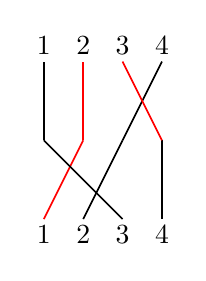
\begin{tikzpicture}
    \draw (0,2+0.2) node {$1$};
    \draw (0.5,2+0.2) node {$2$};
    \draw (1,2+0.2) node {$3$};
    \draw (1.5,2+0.2) node {$4$};
    \draw[semithick, color=red] (0,0) -- (0.5,1);% first line
    \draw[semithick, color=red] (0.5,1) -- (0.5,2);% first line
    \draw[semithick] (0.5,0) -- (1,1);% second line
    \draw[semithick] (0,1) -- (0,2);% second line
    \draw[semithick] (1,0) -- (0,1);% third line
    \draw[semithick] (1,1) -- (1.5,2);% third line
    \draw[semithick] (1.5,0) -- (1.5,1);% fourth line
    \draw[semithick, color=red] (1.5,1) -- (1,2);% fourth line
    \draw (0,-0.2) node {$1$};
    \draw (0.5,-0.2) node {$2$};
    \draw (1,-0.2) node {$3$};
    \draw (1.5,-0.2) node {$4$};
  \end{tikzpicture}
  \caption{The wiring diagram for the permutation  $3\bar{1}24 \circ 1\bar{2}\bar{4}3$. You can see that there is a permutation that changes its sign two times.}
  \end{center}
\label{fig:wiring_snB}
\end{figure}

We introduce the hyperoctahedral group $S_n^B$ as being the group of signed permutations of $\big[n\big] := \{1, 2, \dots, n\}$. The group set is $\{1,2,\dots,m,\bar{1}, \bar{2},\dots, \bar{n}\}$. We have a new generator $t$, that will change the sign of an element. In figure \ref{fig:wiring_snB} we can see an example of permutation within this group. This is a Coxeter group and its diagram is:

\begin{center}
  \dynkin[Coxeter, labels={s_n, s_{n-1}, s_{n-2},s_2,s_1, t}, edge length=.50cm, gonality=n ]{B}{}
\end{center}

Given a Coxeter system $(W,S)$, we can define $T := \{wsw^{-1} |\ s\in S, w \in W\} \subseteq W$ where $s$ are simple reflections.

\begin{definition}
  Given $W \to S_T^B : w \to \pi_w$, $t\in T$ and $s\in S$:

  \begin{equation}
    \pi_s(t) := \left \{
    \begin{array}{c @{} c}
        -s \quad &\text{if } t = s \\
        sts \quad &\text{if } t \neq s \\
    \end{array}\right.
  \end{equation}
\end{definition}
This application is a bijection because its inverse is itself ($\pi_s(\pi_s(s)) = s$):

\begin{equation}
  \pi(\pi_s(t)) = \left \{
  \begin{array}{c @{} c}
      \pi_s(-s) \quad &\text{if } t = s \\
      \pi_s(tsts) \quad &\text{if } t \neq s \\
  \end{array}\right.
\end{equation}
We clearly see that $\pi_s(sts) = s(sts)s = t$ and $\pi_s(-s) = -\pi_s(s) = -s$.

%\begin{equation}

%\end{equation}


	\begin{theorem}
		The application $\pi$ that we defined on the set of generators $S$ of the Coxeter system $(W,S)$, extends uniquely to an injective homomorphism $\pi\fctt{W}{S^B_T}$
	\end{theorem}
	\begin{proof}
		First of all, we need to show that the extension of $\pi$ is well defined. It was clear, due to the definition of $\pi$ on $S$ that for every $s\in S$, the application $\pi_s\in S^B_T$. Indeed, for every $t\in T$ we had that $\pi_s(t)\in T\cup \ub{T}$ and we had that $\pi_s$ defined a bijection on $T\cup \ub{T}$. Now, we need to check that its extension on all of $W$ is still well defined. We need to check 2 things. First, we need to check that $\forall w\in W$ the application $\pi_w\in S_T^B$. But, since we extended $\pi$ from $S$ to $W$ to be a group morphism, we know that $\pi_w$ is by definition the composition of $\pi_s$ for some $s\in S$ and thus is an element of $S_T^B$. Secondly, we need to check that this application $\pi_w$ does not depend on the writing of $w\in W$. To this aim, let us take $t\in T$ and let $w=s_1s_2..s_k$ for some $s_i\in S$ (this is the form of every element of $W$ since $s_i=s_i^{-1}$ for all $i$). Since, we want $\pi$ to be a homomorphism, we have that :
		\begin{equation}\label{equation donnant la form explicite de pi}
		\begin{split}
		\pi_w(t)\qq&=\qq \pi_{s_1}\circ\pi_{s_2}\circ ... \circ \pi_{s_k}(t)\\
		&=\qq \pi_{s_1}\circ\pi_{s_2}\circ ... \circ \pi_{s_{k-1}}(\pm s_kts_k)\q\q\\
		& \q\q (\mbox{with }-\mbox{ iff }s_kts_k=s_k\iff t=s_k)\\
		&=\qq \pi_{s_1}\circ\pi_{s_2}\circ ... \circ \pi_{s_{k-2}}(\pm\pm s_{k-1}s_kts_ks_{k-1})\q\q\\
		& \q\q(\mbox{with }-\mbox{ iff }s_{k-1}s_kts_ks_{k-1}=s_{k-1}\iff t=s_ks_{k-1}s_k)\\
		&=\qq \pi_{s_1}\circ\pi_{s_2}\circ ... \circ \pi_{s_{k-3}}(\pm\pm\pm s_{k-2}s_{k-1}s_kts_ks_{k-1}s_{k-2})\q\q \\
		&\q\q (\mbox{with }-\mbox{ iff }s_{k-1}s_kts_ks_{k-1}=s_{k-1}s_{k-2}\iff t=s_ks_{k-1}s_{k-2}s_{k-1}s_k)\\
		&=\q\q \q\vdots\q\q \q\vdots\q\q \q\vdots\q\q \q\vdots\q\q \q\vdots\q\q \q\vdots\q\q \q\vdots\q\q \q\vdots\q\q \q\vdots\\
		&=\qq \pm\pm \dots \pm s_1s_2...s_kts_ks_{k-1}... s_1\q\q\\
		& \q\q (\mbox{with }-\mbox{ iff }s_1...s_{k-1}s_kts_ks_{k-1}...s_1=s_{1}\iff t=s_k...s_2s_1s_2...s_k)\\
		&=\mbox{sgn}_w(t)\qq wtw^{-1}
		\end{split}
		\end{equation}
		where the function $\mbox{sgn}_w(t)$ is a sign function counting the number of times we have an index $l\in \{1,2,...k\}$ such that $t=s_k...s_{l-1}s_l s_{l-1}...s_k$. Namely :
		\begin{equation}
		 \mbox{sgn}_w(t)\qq=\qq (-1)^{\# \{1\leq l\leq k\qq :\qq t=s_k...s_{l-1}s_l s_{l-1}...s_k\}}
		\end{equation}
		As we will show just after this sign function does not depend of the writing of $w\in W$ in the Coxeter system $(W,S)$.

		But first, let us get some intuition about what this sign function is counting with a visual representation that we have seen before in the chapter: wiring diagrams. In figure \ref{fig:wiring_sign} you can find an example for $S_n$.
		\begin{figure}

		  \begin {center}
		  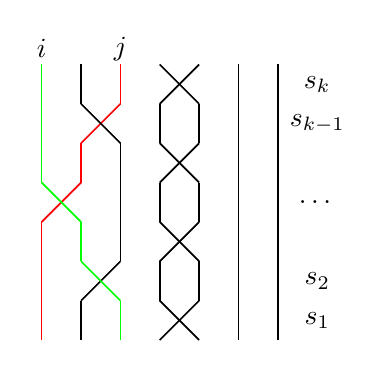
\begin{tikzpicture}

				\def\xa{0}
				\def\xb{0.5}
				\def\xc{1}
				\def\xd{1.5}
				\def\xe{2}
				\def\xf{2.5}
				\def\xg{3}

				%first level
				\draw[semithick, color=red] (\xa,0) -- (\xa,0.5);
				\draw[semithick] (\xb,0) -- (\xb,0.5);
				\draw[semithick, color=green] (\xc,0) -- (\xc,0.5);
				\draw[semithick] (\xd,0) -- (\xe,0.5);
				\draw[semithick] (\xe,0) -- (\xd,0.5);
				\draw[semithick] (\xf,0) -- (\xf,0.5);
				\draw[semithick] (\xg,0) -- (\xg,0.5);

				%second level
				\draw[semithick, color=red] (\xa,0.5) -- (\xa,1);
				\draw[semithick] (\xb,0.5) -- (\xc,1);
				\draw[semithick, color=green] (\xc,0.5) -- (\xb,1);
				\draw[semithick] (\xd,0.5) -- (\xd,1);
				\draw[semithick] (\xe,0.5) -- (\xe,1);
				\draw[semithick] (\xf,0.5) -- (\xf,1);
				\draw[semithick] (\xg,0.5) -- (\xg,1);

				%third level
				\draw[semithick, color=red] (\xa,1) -- (\xa,1.5);
				\draw[semithick, color=green] (\xb,1) -- (\xb,1.5);
				\draw[semithick] (\xc,1) -- (\xc,1.5);
				\draw[semithick] (\xd,1) -- (\xe,1.5);
				\draw[semithick] (\xe,1) -- (\xd,1.5);
				\draw[semithick] (\xf,1) -- (\xf,1.5);
				\draw[semithick] (\xg,1) -- (\xg,1.5);

				%fourth level
				\draw[semithick, color=red] (\xa,1.5) -- (\xb,2);
				\draw[semithick, color=green] (\xb,1.5) -- (\xa,2);
				\draw[semithick] (\xc,1.5) -- (\xc,2);
				\draw[semithick] (\xd,1.5) -- (\xd,2);
				\draw[semithick] (\xe,1.5) -- (\xe,2);
				\draw[semithick] (\xf,1.5) -- (\xf,2);
				\draw[semithick] (\xg,1.5) -- (\xg,2);

				%fifth level
				\draw[semithick, color=green] (\xa,2) -- (\xa,2.5);
				\draw[semithick, color=red] (\xb,2) -- (\xb,2.5);
				\draw[semithick] (\xc,2) -- (\xc,2.5);
				\draw[semithick] (\xd,2) -- (\xe,2.5);
				\draw[semithick] (\xe,2) -- (\xd,2.5);
				\draw[semithick] (\xf,2) -- (\xf,2.5);
				\draw[semithick] (\xg,2) -- (\xg,2.5);

				%sixth level
				\draw[semithick, color=green] (\xa,2.5) -- (\xa,3);
				\draw[semithick, color=red] (\xb,2.5) -- (\xc,3);
				\draw[semithick] (\xc,2.5) -- (\xb,3);
				\draw[semithick] (\xd,2.5) -- (\xd,3);
				\draw[semithick] (\xe,2.5) -- (\xe,3);
				\draw[semithick] (\xf,2.5) -- (\xf,3);
				\draw[semithick] (\xg,2.5) -- (\xg,3);

				%seventh level
				\draw[semithick, color=green] (\xa,3) -- (\xa,3.5);
				\draw[semithick] (\xb,3) -- (\xb,3.5);
				\draw[semithick, color=red] (\xc,3) -- (\xc,3.5);
				\draw[semithick] (\xd,3) -- (\xe,3.5);
				\draw[semithick] (\xe,3) -- (\xd,3.5);
				\draw[semithick] (\xf,3) -- (\xf,3.5);
				\draw[semithick] (\xg,3) -- (\xg,3.5);

				\draw (\xa,3.7) node {$i$};
		   	\draw (\xc,3.7) node {$j$};

				\draw (\xg+0.5,3.25) node {$s_k$};
				\draw (\xg+0.5,2.75) node {$s_{k-1}$};
				\draw (\xg+0.5,1.75) node {\ldots};
				\draw (\xg+0.5,0.75) node {$s_2$};
				\draw (\xg+0.5,0.25) node {$s_1$};

		  \end{tikzpicture}
		  \caption{ A wiring diagram for a word $w \in W$ of the coxeter group $S_n$. You can see that $sgn_w(t)$ with $t = (i,j)$ equals 1 because there is only one crossing between the wires that begin at $i$ and $j$.}
		  \end{center}
		\label{fig:wiring_sign}
		\end{figure}



		We are now going to use equation \ref{equation donnant la form explicite de pi} to prove that $\pi$ is a well defined homomorphism which is equivalent to show that the sign function does not depend on the writing of $w\in W$ in the Coxeter system $(W,S)$. It suffices to show that all the relations we had in $(W,S)$ are satisfied by their image in $S^B_T$. I.e. let us take $s,s'\in S$, we want to show that :
		\begin{equation}\label{equation provant que les relations sont preserves par pi}
		(\pi_s\circ \pi_{s'})^{m(s,s')}\qq=\qq \mbox{Id}_{S^B_T}
		\end{equation}
		Since $(ss')^{-1}=s's$, equation \ref{equation donnant la form explicite de pi} gives for all $t\in T$ :
		\begin{equation}
		(\pi_s\circ \pi_{s'})^{m(s,s')}(t)\qq=\qq \pm\qq (ss')^{m(s,s')}t(s's)^{m(s,s')}\qq=\qq \pm \qq et e\qq=\qq\pm \qq  t
		\end{equation}
		But the sign must be $+$ as here, $w=(ss')^{m(s,s')}$ and therefore we look at :
		\begin{equation}
		{\# \{1\leq l\leq m(s,s') \qq :\qq t=\underset{2l-1 \mbox{ characters}}{\underbrace{s'ss'...s'ss'}}\}}
		\end{equation}
		Which must be even. Indeed, if for some $l\leq m(s,s')/2$ we have :
		\begin{itemize}
			\item if $ m(s,s')$ is even :
			\begin{equation}
			t\qq=\qq \underset{2l-1 \mbox{ characters}}{\underbrace{s'ss'...s'ss'}}\qq=\qq\underset{2l-1 + m(s,s') \mbox{ characters}}{\underbrace{s'ss'...s'ss'}}\qq=\qq \underset{2(l+m(s,s')/2)-1 \mbox{ characters}}{\underbrace{s'ss'...s'ss'}}
			\end{equation}
			\item  if $ m(s,s')$ is odd :
			\begin{equation}
			t\qq=\qq \underset{2l-1 \mbox{ characters}}{\underbrace{s'ss'...s'ss'}}\qq=\qq\underset{2l-1 +m(s,s') \mbox{ characters}}{\underbrace{s'ss'...s'ss'}}\qq=\qq \underset{2((m(s,s')-1)/2+l)+1 \mbox{ characters}}{\underbrace{s'ss'...s'ss'}}
			\end{equation}
		\end{itemize}
	This shows that if one index is counted below $m(s,s')/2$ then there exists an other index counted strictly upper than $m(s,s')/2$ and vis versa. Thus the set must be even and the sign must be $+$. Therefore, equation \eqref{equation provant que les relations sont preserves par pi}, is proved and we $\pi$ is a well defined morphism.

	It remains to show that the extension of $\pi$ is injective. Let $u,v\in W$ be such that $\pi_u=\pi_v$ then, we have that :
	\begin{equation}
	\pi_{uv^{-1}}\qq=\qq \pi_u\circ \pi_{v^{-1}}\qq=\qq \mbox{Id}_{S_T^B}\qq=\qq  \pi_e
	\end{equation}
	Thus, we just need to show that if $w\in W$ is such that $\pi_w=\pi_e$ then $w=e$ to prove the injectivity of $\pi$. Now, let us take $w\in W$ such that $\pi_w=\pi_e$ and let us suppose absurdly that $w\not=e$ then, there exists $k\geq 1$ such that $w=s_1...s_k$ is the shorter way possible to write $w\in W$ then (meaning that $k$ is the smallest possible) :
	\begin{equation}\label{equation pour la contradiction par signe de sk}
	\begin{split}
		s_k\qq=\qq\pi_e(s_k)\qq&=\qq \pi_w(s_k)\qq =\qq\mbox{sgn}_w(s_k)\qq s_1...s_{k-1}s_ks_ks_ks_{k-1}...s_1\qq\\
		&=\qq\mbox{sgn}_w(s_k)\qq s_1...s_{k-1}s_ks_{k-1}...s_1
	\end{split}
	\end{equation}
	But $\mbox{sgn}_w(s_k)=-1$ because :
	\begin{equation}
	\{1\leq l\leq k\qq :\qq t=s_k...s_{l-1}s_l s_{l-1}...s_k\}\qq=\qq \{k\}
	\end{equation}
	Indeed, for $l=k$ we have $s_k=s_k$. But if $l\not=k$ and if we had :
	\begin{equation}
	s_k=\qq s_k..s_l..s_k
	\end{equation}
	Then we would have :
	\begin{equation}
	s_{l-1}...s_ks_k\qq=\qq s_l...s_k
	\end{equation}
	Therefore, we would have a contradiction with the minimality of $k$ since :
	\begin{equation}
	\begin{split}
	w&=s_1...s_ls_{l-1}s_l...s_k\qq\\
	&=\qq s_1...s_{l-1}s_{l-1}...s_ks_k\qq\\
	&=\qq s_1..s_{l-2}s_{l+1}...s_{k-1}\qq\\
	&=\qq s_1...s_{l-2}s_{l+11}...s_{k-1}
	\end{split}
	\end{equation}
	which is a shorter way to write $w$. Therefore, we have that $\mbox{sgn}_w(s_k)=-1$ and thus equation \ref{equation pour la contradiction par signe de sk} gives :
	\begin{equation}
			s_k\qq=\qq -\qq  s_1...s_{k-1}s_ks_{k-1}...s_1
	\end{equation}
	which is a contradiction due to the presence of a sign.\qed
	\end{proof}


	We are now going to define the notions of \tg{parity} and \tg{length} of an element in a Coxeter group.
	\begin{definition}
		Let $(W,S)$ be a Coxeter system, and let $w\in W$, then we say that $w=s_1...s_k$ $(s_l\in S)$ is :
		\begin{itemize}
			\item \tg{even} when $k$ is even.
			\item \tg{odd} when $k$ is odd.
		\end{itemize}
	This is what we call the \tg{parity} of $w\in W$.
	\end{definition}
\begin{remark}
	As all the relations of a Coxeter group involve a pair number of $s\in S$ we see that the parity of an element $w\in W$ doesn't depend on its writing in $W$.
\end{remark}
The set of even elements of a Coxeter system $(W,S)$ is a subgroup of $W$ called the \tg{alternating} subgroup.
\begin{remark}
	When $S_n$ is seen as a Coxeter group with $S=\{s_1...s_{n-1}\}$ and the Coxeter matrix $m(s_i,s_{i+1})=3$ and $m(s,s')=2$ for every other couple $(s,s')\not=(s,s)$ see that the two notions of alternating group coincide.
\end{remark}
\begin{definition}
	Let $(W,S)$ be a Coxeter system, the \tg{length} $l(w)$ of an element $w\in W$ is defined as the smallest integer $k\in \N$ such that there exists $s_1,...,s_k\in S$ with $w=s_1...s_k$.
\end{definition}
The purpose of what follows is to prove the following theorem :
\begin{theorem}\label{theorem sur le calcul des longueurs}
	Let $(W,S)$ be a Coxeter system, and let $w\in W$ then :
	\begin{equation}
	l(w)\qq=\qq \#\{t\in T\qq :\qq \mbox{sgn}_{w^{-1}}(t)=-1\}
	\end{equation}
\end{theorem}
\begin{example}
	In the case where $W=S_n$ with the common representation, $l(w)$ is exactly the number of inversions of $w^{-1}$ which is exactly the same as the number of inversions of $w$ itself.
\end{example}
Before proving this theorem, we focus our attention on some lemma :
\begin{lemma}\label{le lemme de la longueur de tw}
	Let $(W,S)$ be a Coxeter system and let $w\in W$, $t\in T$ then :
	\begin{equation}
	\mbox{sgn}_{w^{-1}}(t)=-1\q \iff \q l(tw)\qq<\qq l(w)
	\end{equation}
\end{lemma}
\begin{proof}
	Let's suppose that $\mbox{sgn}_{w^{-1}}(t)=-1$ and let $w=s_1...s_k$ with $k=l(w)$ then $w^{-1}=s_k...s_1$. We know that there must exist some $1\leq l\leq k$ such that $t=s_1...s_l..s_1$ but then :
	\begin{equation}
	\begin{split}
	tw\qq&=\qq s_1s_2...s_l...s_1\qq q_1s_2...s_ls_{l+1}...s_k\\
	&=\qq s_1s_2...s_{l-1}s_{l+1}...s_k\\
	&=\qq s_1s_2...\hat{s_l}...s_k
	\end{split}
	\end{equation}
	from which we conclude that $l(tw)\leq k-1\qq <\qq k=l(w)$ and the first implication is proven.\\
	Conversely, let's suppose that $l(tw)<l(w)$ then, as $tt=e$ we have that :
	\begin{equation}
	l(tw)\qq <\qq l(ttw)\qq \Rightarrow l(ttw)\not<l(tw)
	\end{equation}
	Therefore, the first implication that we already proved, gives us by taking $\tilde{w=tw}$ that :
	\begin{equation}
	\mbox{sgn}_{w^{-1}t}(t)=+1
	\end{equation}
	Thus,
	\begin{equation}
	\pi_{(tw)^{-1}}(t)\qq=\qq +1 \qq (tw)^{-1}\qq t\qq(tw)\qq=\qq w^{-1}tw
	\end{equation}
	But, by the fact that $\pi$ is a morphism we have that :
	\begin{equation}\label{pi est un homo}
	\pi_{(tw)^{-1}}\qq=\qq\pi_{w^{-1}t}\qq=\qq =\pi_{w^{-1}}\circ\pi_t
	\end{equation}
	Now let's remark that $\forall t\in T$ we have that :
	\begin{equation}
	\pi_t(t)\qq=\qq \mbox{sgn}_t(t)\qq ttt\qq=\qq -t
	\end{equation}
	Indeed, let's write $t=s_1...s_kss_k...s_1$ for a $k$ that is minimal. Then it is clear that :
	\begin{equation}\label{le signe de t de t}
	\{1\leq l\leq 2k+1\qq :\qq t=s_1...s_{l-1}s_l s_{l-1}...s_1\}\qq=\qq \{k+1\}
	\end{equation}
	as by the minimality, it can't be true for $l\leq k$ that $t=s_1...s_{l-1}s_l s_{l-1}...s_1$ and as if it is true for some $l= k+1+l'$ with $l'>0$ we have that
	\begin{equation}
	t\qq=\qq s_1s_2...s_kss_k...s_{k-l'+1}s_{k-l'}s_{k-l'+1}...s_kss_k...s_2s_1
	\end{equation}
	Therefore, by multiplying both sides by $s_1s_2...s_ks$ from the right and by $ss_k...s_2s_1$ from the left, we obtain that :
	\begin{equation}
	s\qq=\qq s_k...s_{k-l'+1}s_{k-l'}s_{k-l'+1}...s_k
	\end{equation}
	Therefore, by replacing $s$ in $t$ we have that :
	\begin{equation}
	t\qq=\qq s_1...s_kss_k...s_1\qq=\qq s_1...s_ks_k...s_{k-l'+1}s_{k-l'}s_{k-l'+1}...s_ks_k...s_1\qq=\qq s_1...s_{k-l'}...s_1
	\end{equation}
	which again contradicts the minimality of $k$. Therefore, the equality \eqref{le signe de t de t} is verified and we have that :
	\begin{equation}
	\pi_t(t)\qq=\qq -t
	\end{equation}
	And by computing equality \eqref{pi est un homo} on $t$ we obtain that :
	\begin{equation}
	\begin{split}
	\pi_{(tw)^{-1}}(t)\qq&=\qq \pi_{w^{-1}}\pi_t(t)\qq\\
	&=\qq \pi_{w^{-1}}(-t)\qq\\
	&=\qq -\qq \pi_{w^{-1}}(t)\\
	&=\qq -\mbox{sgn}_{w^{-1}}(t)\qq w^{-1}tw
	\end{split}
	\end{equation}
	And we finally conclude that $\mbox{sgn}_{w^{-1}}(t)=-1$.\qed
\end{proof}

As a Corollary we have the following lemma :
\begin{lemma}[Exchange property]
Let $(W,S)$ be a Coxeter system and let $w=s_1s-2...s_k\in W$ and $t\in T$, then, if $l(tw)<l(w)$ then, there exists some $1\leq l\leq k$ such that :
	\begin{equation}
	tw\qq=\qq s_1s_2...\hat{s_l}... s_k
	\end{equation}
\end{lemma}
\begin{proof}
	By the previous lemma, we know that $\mbox{sgn}_{w^{-1}}t\qq=\qq -1$. Therefore, we know there exists a $1\leq l\leq k$ such that $tw\qq=\qq s_1s_2...\hat{s_l}... s_k$.\qed
\end{proof}
\begin{lemma}
	Let $(W,S)$ be a Coxeter system and let $w=s_1s_2...s_k\in W$, with $k=l(w)$ and let's take $t\in T$. Then, the following are equivalent :
	\begin{enumerate}
		\item $l(tw)<l(w)$
		\item $tw\qq=\qq s_1...\hat{s_l}...s_1$ for some $1\leq l\leq k$
		\item $t=s_1...s_l...s_1$ for some $1\leq l\leq k$
	\end{enumerate}
Moreover, such an $l$ is uniquely determined.
\end{lemma}
\begin{proof}
	By Lemma \ref{le lemme de la longueur de tw} we already know that $(1)$ implies $(2)$. Furthermore, the equivalence between $(2)$ and $(3)$ is a tautology. Let us prove that $(2)$ implies $(1)$. Indeed, if $tw\qq=\qq s_1...\hat{s_l}...s_1$ for some $1\leq l\leq k$ then :
	\begin{equation}
	l(tw)\qq \leq \qq k+1\qq <\qq k \qq=\qq l(w)
	\end{equation}
	which is $(1)$. It remains to show that this $l$ appearing in property $(2)$ and $(3)$ is unique under the hypothesis that $k=l(w)$. Let us define $t_i=s_1s_2...s_i...s_1$ for all $1\leq i\leq k$. Then, we want to show that  $t_i\not=t_j$ for every $i\not=j$. Let's reason by absurd and suppose the contrary. Therefore, there exists $i<j$ such that $t_i=t_j$. Then,
	\begin{equation}
	\begin{split}
	w\qq&=\qq t_it_j\qq w\\
	&=\qq t_is_1...\hat{s_j}...s_k\\
	&=\qq s_1...\hat{s_i}...\hat{s_j}...s_k
	\end{split}
	\end{equation}
	as $i$ was less than $j$. But this is a contradiction with the exchange property applied for $t=t_it_j$. Therefore we needed that $t_i\not=t_j$ for every $i\not=j$. In particular $l$ must be unique.
	\qed
\end{proof}
With all those lemma, we are now ready to prove theorem \ref{theorem sur le calcul des longueurs}.
\begin{proof}
	Let $w=s_1s_2...s_k$ with $k=l(w)$, then $w^{-1}=s_k...s_1$ and due to the previous lemma, we know that :
	\begin{equation}
	\begin{split}
		\#\{t\in T\qq :\qq \mbox{sgn}_{w^{-1}}(t)=-1\}\qq\q\q\q\q\q\q\q \\
		=\qq \# \{t\in T\qq:\qq t=s_1...s_i...s_k\qq \mbox{for some }1\leq l\leq k\}\qq=\qq k\qq =l(w)
	\end{split}
	\end{equation}
	as every of the $t_i=s_1...s_i...s_1$ are different from each other. \qed
\end{proof}


The following theorem describes the writing reduction of a world in a Coxeter group when it's not written in one of its minimal writings.
\begin{theorem}[Deletion property]
Let $(W,S)$ be a Coxeter system and let $w=s_1s_2...s_k$ for some $k$ with $l(w)<k$ then there exists two different indices $1\leq i<j\leq k$ such that :
	\begin{equation}
	w\qq=\qq s_1...\hat{s_i}...\hat{s_j}...s_k
	\end{equation}
\end{theorem}
A consequence is the following proposition :
\begin{proposition}
	Let $(W,S)$ be a Coxeter system and let $w=s_1...s_k$ for some $s_i\in S$ then, if $l(w)<k$ there exists a sub-word $s_{i_1}...s_{i_{l(w)}}$ of $s_1...s_k$ such that $w=s_{i_1}...s_{i_{l(w)}}$.
\end{proposition}
This proposition is used in the following :
\begin{proposition}
	Let $(W,S)$ be a Coxeter system, and let's suppose that $w=s_1s_2...s_k=s_1's_2'...s_k'$ for some $s_i,s_i'\in S$ with $k=l(w) $. Then, \begin{equation}
	\{s_1,s_2...s_k\}\qq=\qq \{s_1',s_2'...s'_k\}
	\end{equation}
\end{proposition}
\begin{remark}
	To be precise, the upper equality is an equality of sets an not of multi-sets. Indeed, as a simple example that the multi-sets can be different, we take the Coxeter group $S_3$ and the permutation $(2,3)(1,2)(2,3)=(1,3)=(1,2)(2,3)(1,2)$. Therefore, we have the multi-sets :
	\begin{equation}
	\{(2,3),(1,2),(2,3)\}\q \mbox{and}\q \{(1,2),(2,3),(1,2)\}
	\end{equation}
\end{remark}
\begin{proof}
	Suppose that the two sets are not equal. Therefore, there exists an $1\leq i\leq k$ minimal such that $s_i\not\in  \{s_1',s_2'...s'_k\}$. Furthermore, by lemma \ref{les equivalences pour tw}\textbf{Bad reference here} we know that :
	\begin{equation}
	\begin{split}
	\{s_1'...s_j'...s_1':j=1,2,...,k\}\qq&=\qq \{t\in T\qq:\qq l(tw)<l(w)\}\qq\\
	&=\qq \{s_1...s_j...s_1:j=1,2,...,k\}
	\end{split}
	\end{equation}
	As those sets are equal, there must be an index $1\leq j\leq k$ such that for our previous $i$ we have :
	\begin{equation}
	s_1...s_i...s_1\qq=\qq s_1'...s_j'...s_1'
	\end{equation}
	In particular, by previous proposition, there exists a sub-word of the right hand side which is of size $1$ and which is equal to $s_i\in W$. Therefore, either $s_i$ is one of the previous $s_1...s_{i-1}$ which would be a contradiction with the minimality of $i$, or $s_i$ is one of the $s_1',...,s_j'$ which is a contradiction with our choice of $i$. Therefore, the two sets must be the same.
\end{proof}

\begin{theorem} [Matsumoto]
Let $W$ be a group and $S \subset W$ a finite subset of generators of $W$ of order $2$. Then the following assertions are equivalent:
\begin{itemize}
\item $(i)$ $(W, S)$ is a Coxeter system.
\item $(ii)$ $(W, S)$ satisfies the exchange property.
\item $(iii)$ $(W,S)$ satisfies the deletion property.
\end{itemize}
\end{theorem}
\begin{proof}
$(i) \Rightarrow (ii)$. This implication has already been shown above.

$(ii) \Rightarrow (iii)$. Let $w= s_1 \ldots s_k$ such that $\ell(w) < k$. Let $i$ be maximal such that $s_i s_{i+1} \ldots s_k$ is not reduced (i.e. $s_{i+1} \ldots s_k$ is reduced). We have $\ell (s_i s_{i+1} \ldots s_k) \le k- i = \ell (s_{i+1} \ldots s_k)$. Now, using exchange property, we obtain $s_i s_{i+1} \ldots s_k = s_{i+1} \ldots \hat{s}_j \ldots s_k$ for some $i+1 \le j \le k$. Therefore, $w = s_1 \ldots s_{i-1} s_i s_{i+1} \ldots s_k = s_1 \ldots s_{i-1} \hat{s}_i s_{i+1} \ldots \hat{s}_j \ldots s_k$ and we have the result (let us note that this implication remains true for weaker hypothesis since we did not use the fact that $S$ is of order $2$).

$(iii) \Rightarrow (ii)$. Let $w= s_1 \ldots s_k$, $k = \ell (w)$, $s\in S$, such that $\ell (s w) = \ell (s s_1 \ldots s_k) \le \ell (w) = \ell (s_1 \ldots s_k ) = k$. So $s s_1 \ldots s_k$ is not reduced. We can apply the deletion property. Suppose that $s w = s s_1 \ldots \hat{s}_i \ldots \hat{s}_j \ldots s_k $ (but $\ell (sw) \le k-1 < l(w)$). So $s s w = s s s_i \ldots \hat{s}_i \ldots {\hat{s}_j} \ldots s_k$. This leads to $\ell (s_1 \ldots ... \hat{s}_i \ldots \hat{s}_j \ldots s_k ) < k$, which is a contradiction, so this case has to be excluded. Hence, we have $s w = \hat{s} s_1 \ldots \hat{s}_i  \ldots s_k $.

$(ii) \Rightarrow (i)$. Using $(ii) \Rightarrow (iii)$, we can assume both $(ii)$ and $(iii)$. Define $m(s,s') = \text{order of $ss'$ in $W$, for all $s,s' \in S$}$. Let $(\tilde{W}, S)$ be the Coxeter group associated to $m$. Clearly, $\phi: \tilde{W} \mapsto W, s \to s$ is a surjective homomorphism. We need to show that $\phi$ is also injective. Let $s_1 \ldots s_m = e$ in $W$. By the deletion property, $m$ is even, say $m=2k$. So we can write our relation on the form
\begin{equation}
s_1 \ldots s_k = s'_1 \ldots s_k'
\label{relation}
\end{equation} where $s_1' = s_{2k}$, $\ldots$ $s_k' = s_{k+1}$. We must now prove that \eqref{relation} is a consequence of the pairwise relations $(ss')^{m(s,s')} = e$. The proof is done by induction on $k$, the case $k = 1$ being trivially correct.
\begin{itemize}
\item \underline{Case 1:} Suppose $w := s_1 \ldots s_k$ is not reduced. By deletion property, there exists a position $1 \le i <k$ such that $s_{i+1} s_{i+2} \ldots s_k$ is reduced but $s_i s_{i+1} s_{i+2} ...s_k$ is not. By the exchange property, we then have that $s_{i+1} s_{i+2} \ldots s_k = s_i s_{i+1} \ldots \hat{s}_j \ldots s_k$ for some $i < j \le k$. This relation is of length $<2k$ and hence fine. Plugging this result into \eqref{relation} gives $s_1 \ldots s_i s_i s_{i+1} \ldots \hat{s}_j \ldots s_k = s_1' s_2' \ldots s'_k$. The factor $s_i s_i$ can be deleted, leaving a relation of length $<2k$. Hence the relation \eqref{relation} is fine.
\item \underline{Case 2:} Suppose $w = s_1 \ldots s_k$ is reduced, $k = \ell (w)$. We can assume that $s_1 \neq s_1'$ (otherwise the relation \eqref{relation} is equivalent to a shorter relation). We have $\ell (s_1' s_1 s_2 \ldots s_k) = \ell (s_1' s_1' s_2' \ldots s_k') = \ell( s_2' \ldots s_k')  \le k-1 < \ell (s_1 \ldots s_k)$. Using exchange property, we have $s_1' s_1 \ldots s_k = s_1 \ldots \hat{s}_i \ldots s_k$ for some $i$. Hence, $s_1 \ldots \hat{s}_i \ldots s_k = s_2' \ldots s'_k$.

If $i<k$, then $s_1' s_1 s_2 \ldots s_{k-1} = s_1 \ldots \hat{s}_i \ldots s_{k-1}$. So $s_1' s_1 s_2 \ldots s_{k-1} s_k = s_1 \ldots \hat{s}_i \ldots s_{k-1} s_k$. Hence, $s_1' s_1 \ldots s_k = s_2' \ldots s_k$ is a consequence of Coxeter relations.

If $i=k$, we have to work a little bit harder. We have $s_1' s_1 \ldots s_{k-1} = s_1' s_2' \ldots s_k' $. Thus it will suffice to show that $s_1 s_1 \ldots s_{k-1} = s_1 s_2 \ldots s_k$ is a consequence of Coxeter relations. Applying recursively the rule, we have $s_1 s_1' s_1 \ldots s_{k-2} = s'_1 s_1 \ldots s_{k-1}$ $\Rightarrow$ $s_1' s_1 s'_1 s_1 \ldots s_{k-3} = s_1 s_1' s_1 \ldots s_{k-2}$ $\Rightarrow$ $\ldots$ Thus in the end, the question will be reduced to the relation $s_1 s_1' s_1 s_1' \ldots = s_1' s_1 s_1' s_1 \ldots$, which is of course a consequence of the Coxeter relation $(s_1 s_1')^{m(s,s')}= e$.


\end{itemize}

\end{proof}


\begin{example}
The group $S_n$ can be generated by transpositions, which are order $2$ elements. Using the above theorem, we conclude that $S_n$ is actually a Coxeter group.
\end{example}

\section{Geometric representation}

Let $(W, S)$ be a Coxeter system, $S = \{s_1, \ldots s_n \}$, $m$ the associated Coxeter matrix. We write $m_{ij} = m(s_i, s_j)$. Let $V$ be a $\mathbb{R}$-vector space of dimension $n$, with a basis $\alpha_1, \ldots , \alpha_n$. We consider the symmetric bilinear map
\begin{equation}
\langle \cdot, \cdot \rangle : V \times V \mapsto \mathbb{R}
\end{equation} defined through
\begin{equation}
\langle \alpha_i , \alpha_j \rangle = \left \{
\begin{array}{c @{} c}
    &- \cos \left(\frac{\pi}{m_{ij}} \right) \quad \text{if } m_{ij} < + \infty \\
    &-1 \quad ~~~~~~~~~~~~~\text{if } m_{ij} = + \infty \\
\end{array}
\right.
\end{equation} Note that $\langle \cdot, \cdot \rangle$ is not positive definite in general.

\begin{proposition}
The following map extends to a homomorphism:
\begin{equation}
W \mapsto GL(V), s_i \to \sigma_i
\end{equation} where $\sigma_i :v \to  v - 2 \langle v, \alpha_i \rangle \alpha_i$.
\end{proposition}

\begin{remark}
We have $\sigma_i (\alpha_i) = \alpha_i - 2 \langle \alpha_i, \alpha_i \rangle \alpha_i = - \alpha_i$. Thus, if $v\in V$ is such that $\langle v, \alpha_i \rangle = 0$, then $\sigma_i (v) = v$. Therefore, if $\langle \cdot, \cdot \rangle$ was positive definite, $\sigma_i$ would be interpreted as a reflexion through the hyperplane orthogonal to $\alpha_i$.
\end{remark}

\begin{proof}
First, let us show that $\sigma_i$ is invertible for all $i$. We have $\sigma^2_i (v) = \sigma_i (v) - 2 \langle v, \alpha_i \rangle \sigma_i (\alpha_i) = v - 2  \langle v, \alpha_i \rangle \alpha_i + 2  \langle v, \alpha_i \rangle \alpha_i = v$.

Now, let us show that $(\sigma_i \sigma_j)^{m_{ij}} = Id_V$. For $i\neq j$, define $V_{ij} = \text{Span}_\mathbb{R} ( \{ \alpha_i , \alpha_j \} )$. Furthermore, $V_{ij}^\perp = \{ v\in V | \langle v, \alpha_i \rangle = 0, \langle v, \alpha_j \rangle = 0 \}$. Before proceeding, we show the following lemma:

\begin{lemma}
$V = V_{ij} \oplus V_{ij}^\perp$ if $m_{ij} < + \infty$.
\end{lemma}

\begin{proof}
Let $v \in V$. We want to find $\lambda_i, \lambda_j \in \mathbb{R}$ such that $\tilde{v} = \lambda_i \alpha_i + \lambda_j \alpha_j \in V_{ij}$ and $v - \tilde{v} \in V_{ij}^\perp$. We have
\begin{equation}
\begin{split}
\langle \tilde{v}, \alpha_i \rangle &= \lambda_i \langle \alpha_i , \alpha_i \rangle + \lambda_j \langle \alpha_i, \alpha_j \rangle \\
&= \lambda_i + C \lambda_j
\end{split}
\end{equation} where $C = \langle \alpha_i, \alpha_j \rangle = - \cos \left( \frac{\pi}{m_{ij}} \right)$. Furthermore,
\begin{equation}
\langle \tilde{v}, \alpha_j \rangle = \lambda_i C + \lambda_j
\end{equation} Since
\begin{equation}
\det \begin{pmatrix}
1 & C \\
C & 1
\end{pmatrix} = 1 - C^2 = 1 - \cos^2 \left( \frac{\pi}{m_{ij}} \right) \neq 0,
\end{equation} if $m_{ij} < + \infty$. Therefore, we can find unique $\lambda_i$ and $\lambda_j$ such that
\begin{equation}
\langle \tilde{v} , \alpha_i \rangle = \langle v, \alpha_i \rangle \quad \text{and} \quad \langle \tilde{v} , \alpha_j \rangle = \langle v, \alpha_j \rangle
\end{equation}
\end{proof}

Now let us come back to the proof of the proposition. Using the lemma, we have $v = \tilde{v} + (v- \tilde{v})$ such that $\langle v - \tilde{v} , \alpha_i \rangle = 0 = \langle v - \tilde{v}, \alpha_j \rangle = 0$. Hence $\sigma_i (v - \tilde{v}) = v- \tilde{v} - 2 \langle v - \tilde{v} , \alpha_i \rangle \alpha_i = v- \tilde{v}$ and $\sigma_j (v-\tilde{v}) = v - \tilde{v}$. In the basis $\{ \alpha_i, \alpha_j \}$ of $V_{ij}$, the matrix associated to $\sigma_i$ is given by
\begin{equation}
\begin{pmatrix}
-1 &-2 C \\
0 & 1
\end{pmatrix}
\end{equation} In fact, we have $\sigma_i (\alpha_i) = -\alpha_i$ and $\sigma_j (\alpha_j ) = \alpha_j - 2 C \alpha_i$. Similarly, the matrix associated to $\sigma_j$ is given by
\begin{equation}
\begin{pmatrix}
1 & 0 \\
-2C & -1
\end{pmatrix}
\end{equation} Therefore,
\begin{equation}
(\sigma_i) (\sigma_j) = \begin{pmatrix}
-1 &-2 C \\
0 & 1
\end{pmatrix} \begin{pmatrix}
1 & 0 \\
-2C & -1
\end{pmatrix} = \begin{pmatrix}
-1 + 4 C^2 & 2C \\
-2 C & -1
\end{pmatrix}
\end{equation} The characteristic polynomial $P$ of this matrix is given by $P(t) = t^2 - (-2 + 4 C^2 ) t + 1$.The roots are given by $t_\pm = \cos \left(\frac{2 \pi}{m_{ij}} \right) \pm i \sin \left( \frac{2 \pi}{m_{ij}} \right)$. This characterizes a rotation of $2 \pi / m_{ij}$. So, the order of $\sigma_i \sigma_j$ is given by $m_{ij}$. 

\end{proof}

\section{Combinatorial representation}

As explained in the first part of this chapter, Coxeter groups can also be viewed as combinatorial objects. In this section, we recall some concepts of combinatorics.

\begin{definition}
  A poset is a tuple $(P, \leq)$ where $P$ is a set and $\leq$ is a binary relation such that:

  \begin{itemize}
    \item $x \leq x\ \ \ \forall x \in P$
    \item if $x \leq y$ and $y \leq x$ then $x = y$
    \item if $x \leq y$ and $y \leq z$ then $x \leq z$
  \end{itemize}
\end{definition}

\begin{figure}
  \begin{center}
    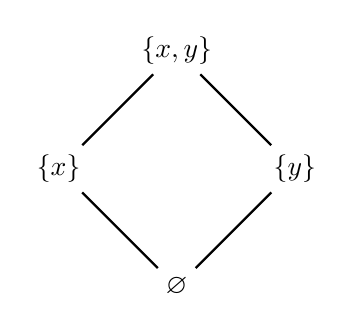
\begin{tikzpicture}[scale=1.5]

  % poset
  \draw (-1cm,0cm) node (v2) {$\{x\}$};
  \draw (1cm,0cm)  node (v3) { $\{y\}$ };
  \draw (0cm,-1cm) node (v4) {$\varnothing$};
  \draw (0cm,1cm)  node (v1) {$\{x,y\}$};

  \draw[thick]  (v1) edge (v2);
  \draw[thick]  (v3) edge (v1);
  \draw[thick]  (v3) edge (v4);
  \draw[thick]  (v2) edge (v4);

  \end{tikzpicture}
\end{center}
\caption{The Hasse Diagram of the poset $(P({x,y}), \subseteq)$.}
\label{fig:hasse}
\end{figure}

A poset can be represented as a Hasse diagram, as shown in the example of figure \ref{fig:hasse}.

\begin{definition}
Let $(W,S)$ be a Coxeter system and $T = \{wsw^{-1} | w \in W, s \in S\}$ a set of reflections. Two elements $u, w \in W$ define a function $u \to v$ if $l(v) > l(u)$ and $v = ut$ for some $t \in T$.
We define an order $w \leq v$ if there exists:

\begin{equation}
u \to u_1 \to u_2 \to \dots \to u_k = v
\end{equation}
\end{definition}
A Bruhat order is a partial order on the elements of a Coxeter group. By using the relation defined in the previous definition, we can have a Bruhat order as shown in figure \ref{fig:bruhat}.

\begin{figure}
\begin{center}

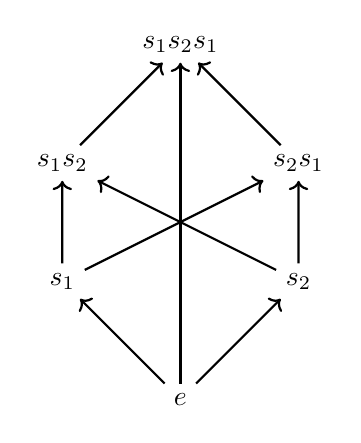
\begin{tikzpicture}[scale=1.5]

  % poset
  \draw (-1cm,0cm) node (v2) {$s_1$};
  \draw (1cm,0cm)  node (v3) {$s_2$ };
  \draw (0cm,-1cm) node (v4) {$e$};
  \draw (-1cm,1cm)  node (v1) {$s_1s_2$};
  \draw (1cm,1cm)  node (v5) {$s_2s_1$};
  \draw (0cm,2cm)  node (v6) {$s_1s_2s_1$};

  \draw[<-, thick]  (v1) edge (v2);
  \draw[->, thick]  (v2) edge (v5);
  \draw[->, thick]  (v3) edge (v1);
  \draw[<-, thick]  (v3) edge (v4);
  \draw[<-, thick]  (v2) edge (v4);
  \draw[->, thick]  (v3) edge (v5);
  \draw[->, thick]  (v1) edge (v6);
  \draw[->, thick]  (v5) edge (v6);
  \draw[->, thick]  (v4) edge (v6);

\end{tikzpicture}
\end{center}
\caption{The Bruhat order $(S_3, \{s_1, s_2\}), T = \{s_1,s_2,s_3,s_4,s_5\}$}
\label{fig:bruhat}
\end{figure}


\begin{theorem}
  Let $u,v \in S_n$, $u \leq v$ if and only if the intersection degree of $u$ is $\leq$ than the one of $v$.
\end{theorem}

\begin{example}
  If we have $35124 \leq 45213$:
  \begin{equation}
    \begin{split}
      3 &\leq 4\\
      35 &\leq 45\\
      135 &\leq 245\\
      1235 &\leq 1245\\
      12345 &\leq 12345
    \end{split}
  \end{equation}
\end{example}

\begin{theorem} [Subword property]
  Let $v = s_1s_2\dots s_q$ reduced word for $v \in W$. Then $u \leq v$ if and only if $u = s_{i_1}s_{i_2} \dots s_{i_k}$ reduced for some $1 \leq i_1 \leq i_2 \leq \dots \leq i_k \leq q$.
\end{theorem}

\begin{proof}
We first prove the \emph{if} part of the theorem. Assume $u \to v$, so $v = ut$ and $l(v) > l(u) = l(utt) = l(vt)$ for some $t \in T$.
By the exchange property:
\begin{equation}
u = vt = s_1s_2\dots \hat{s_i} \dots s_q
\end{equation}
We omit factors iteratively until we have what we want.\\
Second, we prove the \emph{only if} part of the theorem by induction on $l(v) - l(u)$.
If $l(v)-l(u) = 1$ and we have
\begin{equation}
  u = s_1 \dots \hat{s_i} \dots s_q
\end{equation}
with
\begin{equation}
  t = s_q \dots s_i \dots s_q
\end{equation} then $ut = v$ which means that $u \to v$.
If $l(v) - l(u) > 1$ and we have
\begin{equation}
  u = s_1 \dots \hat{s_{a_1}} \dots \hat{s_{a_2}} \dots \hat{s_{a_k}} \dots s_q
\end{equation}
with a minimal $k$ such that $l(v) - l(u) = k$, we take
\begin{equation}
  t = s_q \dots s_{a_k} \dots s_q
\end{equation}
and
\begin{equation}
  ut = s_1 \dots \hat{s_{a_1}} \dots \hat{s_{a_2}} \dots s_{a_k} \dots s_q
\end{equation}
We could have two cases:
\begin{itemize}
  \item Case $l(ut) > l(u)$: \\
  then $l(ut) = l(u) +1$, so $u \to ut$. $l(v)-l(ut) -1$. By induction $ut \leq v$, so $u \leq v$.
  \item Case $l(ut) < l(u)$: \\
 this will be proved impossible by contradiction. By exchange we have
  \begin{equation}
    ut = s_1 \dots \hat{s_{a_1}} \dots \hat{s_{i}} \dots \hat{s_{a_{k-1}}} \dots s_{a_{k}} \dots s_q
  \end{equation}
  If $i > a_k$ and we have
  \begin{equation}
    t = s_q \dots s_1 \dots s_q
  \end{equation}
Then,
  \begin{equation}
    \begin{split}
      vtt &= s_1 \dots s_q (s_q \dots s_{a_k} \dots s_q)(s_q \dots s_i \dots s_q)\\
      &= s_q \dots \hat{s_{a_k}} \dots \hat{s_i} \dots s_q
    \end{split}
  \end{equation}
  which is a contradiction.\\

  If $i < a_k$,
  \begin{equation}
    \begin{split}
      u = utt &= s_1 \dots \hat{s_{a_1}} \dots s_q (s_q \dots \hat{s_{a_k}} \dots s_i \dots \hat{s_k} \dots s_q) (s_q \dots s_{a_k} \dots{s_q})\\
      &= s_1 \dots \hat{s_{a_1}} \dots \hat{s_i} \dots s_{a_k} \dots s_q
    \end{split}
  \end{equation}
You can see that we omit elements to the left of $a_k$, which contradicts the minimality of $a_k$. This proves that the case when $l(ut) < l(u)$ is impossible. Thus, we have proved the first case true which finishes the proof. \qed

\end{itemize}
\end{proof}

From this theorem we can deduct some corollaries.

\begin{corollary}
  $u \leq v$ if and only if $u^{-1} \leq v^{-1}$.
\end{corollary}

\begin{corollary}
  If $u \leq v$ and $l(v) - l(u) = k$, then
  \begin{equation}
    u \leq u_1 \leq u_2 \leq \dots \leq u_k
  \end{equation}
  with $l(u_i) = l(u) + i$ for every $i$.
\end{corollary}

\begin{proof}
Let $v = s_1 \dots s_q$ and $l(v) = q$, $u \leq v$, $l(v) - l(u) = k$ so $l(u) = q-k$. By subword property

\begin{equation}
  u_1 = s_i \dots \hat{s_{a_k}} \dots s_q = u\underset{t}{\underbrace{s_q \dots s_{a_k} \dots s_q}}
\end{equation}
We have then $l(u_1) = l(ut) = l(u)+1$, so $u \to u_1$ which means that $u \leq u_1$. \qed
\end{proof}

\begin{theorem}[Lifting property]
  If $u, v \in W$ and $s \in S$ with $u \leq w$, then $u \leq sw$ and $su \leq w$.
\end{theorem}
\begin{proof}
Take $sw = s_1 \dots s_q$ in a reduced form.
Since $sw \leq w$, $w = ss_1\dots s_q$ is also reduced.
As $u \leq w$, $u$ is a subword of $ss_1 \dots s_q$. If $u$ is a subword of $s_1 \dots s_q$, this corresponds to the theorem. If not,
\begin{equation}
  u = ss_{i_1} \dots s_{i_r}
\end{equation}
is reduced with
\begin{equation}
  1 \leq i_1 \leq i_2 \leq \dots \leq i_r \leq q
\end{equation}
So $su = s_{i_1} \dots s_{i_2}$, which is a contradiction as $u \leq su$. The proof of $su \leq w$ is left to the reader. \qed
\end{proof}

\begin{lemma}
  If $u,v \in W$ then it exists a $w \in W$ such that $u \leq w$ and $v \leq w$.
\end{lemma}

\begin{proof}
  We can prove this by induction on $l(u) + l(v)$. Say $l(u) > 0$:

  We take $s \in S$ such that $l(su)= l(u) - 1$. By induction $l(su) + l(v) < l(u) + l(v)$ so it exists indeed a $w \in W$ such that $su \leq w$ and $v \leq w$. We may have two different cases: if $sw \leq w$ or $w \leq sw$:

  \begin{itemize}
    \item Case $w \leq sw$: by the lifting property, $v \leq sw$ and $u \leq sw$.
    \item Case $sw \leq w$: again by the lifting property, $v \leq w$ and $u \leq w$.
  \end{itemize}

  This proves that there always exists an element that respects the lemma, either $w$ or $sw$. \qed
\end{proof}

\begin{corollary}
If $W$ is finite, there is an unique maximal $w_0 \in W$.
\end{corollary}

\begin{example}
  In $S_n$ we have $w_0 = n(n-1) \dots 1$.
\end{example}

\begin{corollary}
  If there is a $w_0 \in W$ such that $sw_0 \leq w_0$ for all $s \in S$, then $w \leq w_0$ for all $w \in W$ and $W$ is finite.
\end{corollary}

\begin{proof}
  The proof is left to the reader. You may prove this by induction on $l(w)$, by showing that $w \leq w_0$ for all $w \in W$. Then show finitely many choices of $w$.
\end{proof}

This maximal element is very important because it has some properties that relates it with the set of reflections $T$:

\begin{proposition}
  Let $w_0 \in W$ be the maximal element of $W$ and $T_L(w) = \{t\in T |\  l(tw) < l(w)\}$. The following statements are true:
  \begin{itemize}
    \item $w_0^2 = e$
    \item $l(ww_0) = l(w_0) - l(w)$
    \item $T_L(ww_0) = T \setminus T_L(w_0)$
    \item $l(w_0) = |T|$
  \end{itemize}
\end{proposition}

\begin{corollary}
  $u \leq v$ if and only if $vw_0 \leq uw_0$.
\end{corollary}

\section{Parabolic subgroup and parabolic quotient.}
The last ingredients needed to study the link between Coxeter groups and geometry are the notions of Parabolic subgroup and Parabolic quotient. The purpose of this section is to define those two and to investigate some of their basic properties.

\begin{definition}
	Let $(W,S)$ be a Coxeter system and let $J$ be a subset of $S$. Then, we define the \tg{parabolic subgroup} of $W$ associated to $J$ as the group generated by $J$ :
	\begin{equation}
	W_J\qq=\qq <\qq J\qq >\qq \sub \qq W
	\end{equation}
\end{definition}
\begin{remark}
	Before going further, let us remark that for any non empty subset $J\sub S$, the pair $(W_J,J)$ defines a Coxeter system, since it just restricts the set of generators without changing their intertwining relations. We will discuss the proof of this fact in more details in the next proposition.
\end{remark}
\begin{example}
	Let us consider the Coxeter group $S_7$ together with its set of generators  $S=\{s_1,s_2,\dots, s_6\}$ and its classical presentation. If we consider the subset $J=\{s_1,s_2,s_3,s_5,s_6\}$, then, the associated parabolic group is :
	\begin{equation}
	W_J\qq=\qq <\qq <\{s_1,s_2,s_3\}>\qq \cup \qq <\{s_5,s_6\}>\qq >\qq \simeq\qq S_4\qq \times \qq S_3
	\end{equation}
\end{example}
In fact, the phenomena observed in the latest is a general fact when it comes to the symmetric group $S_n$. Take any partition of $n$, meaning any multi index $\alpha=(\alpha_1,\alpha_2,\dots, \alpha_k)$ such that $\s{i=1}{k}\alpha_i=n$, $\alpha_i\in \N\backslash\{0\}$ and consider $J$ as the set containing the $s_i$ for $i\in \lb \alpha_{2j},\alpha_{2j+1}\rb$ for every $j\in \N$ such that $2j\leq n$. We have that :
\begin{equation}
S_\alpha\qq=\qq S_{\alpha_1}\times S_{\alpha_3}\times \dots \times S_{\alpha_{2k+1}}
\end{equation}
where $2k+1$ is the biggest odd index less or equal than $n$.

The following proposition investigate some properties of this parabolic group associated to $J$.
\begin{proposition}
	Le $(W,S)$ be a Coxeter system and let $I,J$ be two subsets of $S$. Then, the following properties hold :
	\begin{enumerate}
		\item The pair $(W_J,J)$ defines a Coxeter system.
		\item If we denote by $l_J$ the length of a coefficient then for every $w\in W_J\sub W$ we have that :
		\begin{equation}
		l_J(w)\qq=\qq l(w)
		\end{equation}
		\item\begin{center}
			$W_I\cap W_J=W_{I\cap J}$
		\end{center}
		\item \begin{center}
			$<\qq W_I\cup W_J\qq >\qq=\qq W_{I\cap J}$
		\end{center}
		\item\begin{center}
			 $W_I=W_J\qq \iff \qq I=J$
		\end{center}
	\end{enumerate}
\end{proposition}
\begin{proof}
	We are going to prove each point separately :
	\begin{enumerate}
		\item Using Matsumata's Theorem, we know that it is enough to prove that the deletion property holds in $(W_J,J)$. But every element of $W_J$ is in particular an element of $W$. Since the deletion property holds in the $W$, we can apply it on the element $w$ and we proved that the deletion property still holds in $(W_J,J)$, which proves it's a Coxeter system.
		\item Let us take $w\in W_J$ and let us write $w=j_1j_2...j_r$ for some $j_i\in J$ and $r=l_J(w)$. Since $w$ is an element of $W$ and $J$ is a subset of $S$ we deduce that $l(w)\leq r$ because our last writing of $w$ in $(W_J,J)$ is also a writing of $w$ in $(W,S)$. Now, let us suppose by absurd that $l(w)\not=l_J(w)$, this means that $l(w)<r$. In particular, this means that we can find by deletion property a subword of $w$ in $(W,S)$ but, since $w$ was written only with element of $J$, this subword contains only elements of $J$. Therefore, we also reduced the word $w$ in $(W_J,J)$ which is a contradiction with the fact that $r=l_J(w)$.
		\item We prove this equality in two inclusions. The inclusion $W_{I\cap J}\sub W_I\cap W_J $ is clear from the definition of group generated by a set. Now let us show the opposite inclusion. Let $w\in W_I\cap W_J$ and let $j_1j_2...j_q=w=i_1i_2...i_q$ be two reduced writing of $w$ in $(W_J,J)$ and $(W_I,I)$ respectively (let us remark that we can write it as the product of $q$ elements in both $J$ and $I$ because of the first second point of the proposition which asserts that $l_J(w)=l(w)=l_I(w)$). Since the equality of the two writings hold in $W$ and since we already saw as a consequence of the deletion property that two reduced writing of $w$ in $(W,S)$ are made with the same set of element we obtain that as a set :$\{i_1,...,i_r\}=\{j_1,...j_r\}$. Therefore, we deduce that $\{i_1,...,i_r\}=\{j_1,...j_r\}\sub I\cap J$ and $w$ is in the subgroup generated by $I\cap J$.
		\item This point is clear since it is true for any subsets $I,J$ of a group $W$ that the union of the group generated by $I$ and $J$ respectively is the group generated by the union $I\cup J$.
		\item The implication $(\Leftarrow)$ is obvious. When it comes to the implication $(\Rightarrow)$, let us suppose by absurd that $I\not=J$ and let us take any $i\in I\backslash J$. Since $i\in I\sub W_I=W_J$ we obtain that $i$ can be written in terms of elements of $J$. Since $i$ is a reduced word this means that $i$ can be written in terms of elements of $J$ with only one element $j$. Furthermore, as a consequence of the deletion property, we know that $\{i\}=\{j\}$ and therefore $i=j\in J$, which is a contradiction.
	\end{enumerate}
\end{proof}
\begin{definition}
	Let $(W,S)$ be a Coxeter system and let $J\sub S$ then, we define its parabolic quotient as the space :
	\begin{equation}
	W^J\qq=\qq\{w\in W\qq \lvert\qq wj>w\qq \mbox{for all }j\in J\}
	\end{equation}
\end{definition}

As we will see later, this parabolic quotient $W^J$ associated to $J$ is a set containing every of the left coset representatives of the parabolic subgroup $W_J$ in $W$. Unfortunately, this parabolic quotient is usually not a group.


The following proposition gives a second point of view of this parabolic quotient :
\begin{proposition}
	Let $(W,S)$ be a Coxeter system and let $J\sub S$ then :
	\begin{equation}
	W^J\qq=\qq\{w\in W\qq :\qq \mbox{no reduced critting of } w \mbox{ ends with an element of }J\}
	\end{equation}
\end{proposition}
\begin{proof}
	We are going to show that the complementary of $W^J$ is the complementary of the above set. Now, to show this set equality we are going to prove two inclusions. The inclusion $\supset$ is clear. Indeed, if a reduced word of $w$ end up with an element $j\in J$ then $l(wj)=l(w)-1$ and therefore, $l(wj)<l(w)$ which proves that $w\in (W^J)^c$. The proof the second inclusion is a straightforward consequence of the exchange property. Indeed, let $w\in (W^J)^c$, and let us consider a writing of $w=s_1...s_k$ such that it is a reduced word of $W$. Since $w\in (W^J)^c$ we know that $wj\leq w$ for some $j\in J$. By an argument of parity since $J\sub S$ the only possibility is that $l(wj)<l(w)$. But, since $J\sub S\sub T$ we can apply the exchange property and we obtain that $wj=s_1...s_{i-1}\check{s_i}s_{i+1}...s_k$ for some index $i\in \{1,2,...,k\}$. In particular, since $j\in J\sub S$, the only possibility is that $i=k$ and that $s_k=j$, otherwise, we would lose more that only one index in the writing of $wj$. Therefore, the reduced writing of $w$ ended with an element of $j\in J$. \qed
\end{proof}
Now, let us consider an explicit example of parabolic subgroup and quotient that will be associated. Let us consider the Coxeter system $(S_3,\{s_1,s_2\})$ and the set $J=\{s_1\}$. Then the associated parabolic subgroup is $W_J=\{e,s_1\}$ and the associated parabolic quotient is $W^J=\{e,s_2,s_1s_2\}$. The following figure represents the Bruhat diagram of this Coxeter group and gives a good intuition of why $W^J$ should be the set of representatives for the coset of $W_J$ in $W$.
\begin{figure}[h]
		\centering
		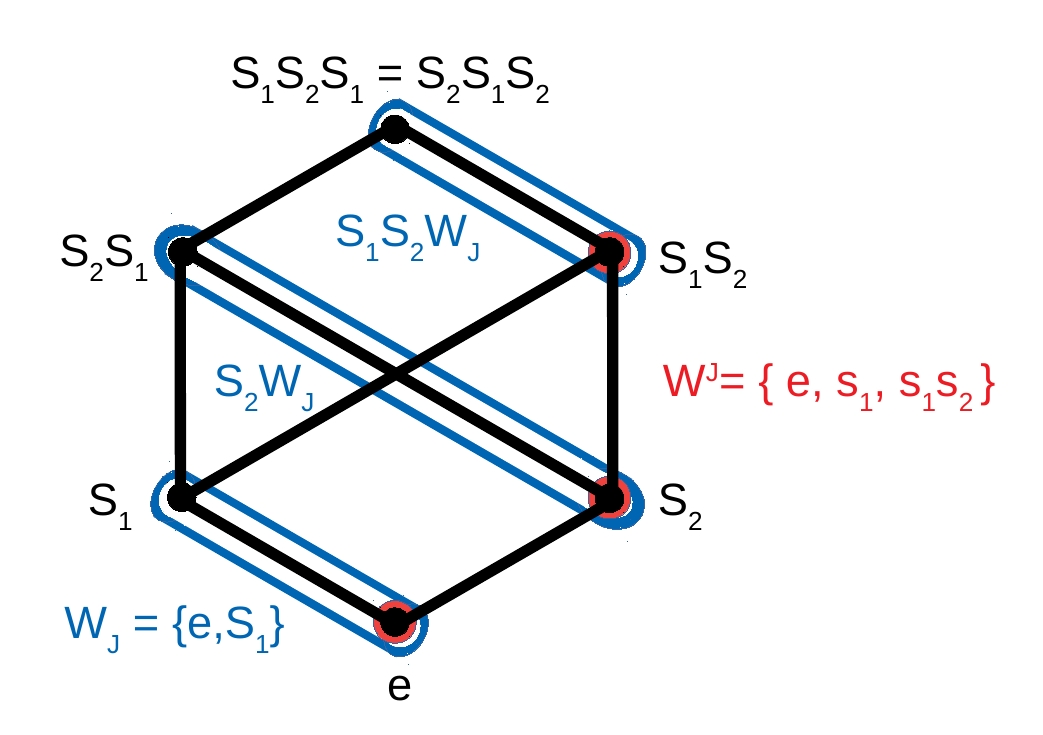
\includegraphics[scale=0.2]{Coxetergroupimagediamand.JPG}
\end{figure}

\begin{proposition}
	Let $(W,S)$ be a Coxeter system, and let $J\sub S$ be a non empty subset of $S$. Then, every element $w\in W$ factors uniquely as a product $w=w^Jw_J$ of an element $w_J$ of the parabolic subgroup $W_J$ and an element $w^J$ of the parabolic quotient $W^J$. Furthermore, $l(w)=l(w_J)+l(w^J)$.
\end{proposition}
\begin{proof}
	Start with a reduced $w$. There are two cases. Either there exists no $j\in J$ such that $w>wj$ and $w\in W^J$ which implies that $w=w\qq e\in w^JW_J$ and we are done. Or there exists some $j_1\in J$ such that $w>wj_1$. In that last case, we can repeat the process. Either there exists no $j\in J$ such that $wj_1>wj_1j$ and $wj_1\in W^J$ therefore $w=wj_1\qq j_1\in w^JW_J$ and we are done. Or there exists some $j_2\in J$ such that $wj_1>wj_1j_2$. In that case, we can again repeat the process. However, this process needs to stop at some point since there is a finite number of letters in any reduced writing of $w$ and since each time a relation $>$ occurs the word becomes at least one letter shorter. In particular, we obtain a sequence :
	\begin{equation}
	w\qq >\qq wj_1\qq >wj_1j_2\qq >\qq ...\qq >\qq wj_1...j_k
	\end{equation}
	for some $k\in\N$ with $k<l(w)$ and some $j_1,...,j_k\in J$, such that $wj_1...j_k\in W^J$. Therefore, we can write $w=wj_1...j_k\qq j_k...j_1\in W^JW_J$ and we obtain what we wanted. Furthermore, since from this process, we observe that $l(wj_1...j_k)=l(w)-k$ we obtain that $l(wj_1...j_k)+l(j_1...j_k)\qq\leq \qq l(w)-k+k=l(w)$. And since $w=w^Jw_J$ we had the opposite inequality $l(w)\leq l(w^J)+l(w_J)$. Therefore, we conclude that $l(w)=l(w^J)+l(w_J)$.

	Now, we need to prove that this decomposition is unique. Let us suppose that $w=w^Jw_J=v^Jv_J$ for some $w^J,v^J\in W^J$ and some $w_J,v_J\in W_J$. Then, $w^J=v^J\qq v_Jw_{J}^{-1}$ and since $W_J$ form a group, we deduce that $v_Jw_{J}^{-1}\in W_J$. Now, chose some reduce writing for $v^J$ in $W$ and some reduce writing for $v_Jw_J^{-1}$ in $W_J$. By deletion, we know that we can reduce the obtained writing of the word $w^J=v^J\qq v_Jw_{J}^{-1}$ and since this reduced word belongs to $W^J$ we know that it can't end with an element of $J$. Therefore, $w^J$ must be a subword of $v^J$. In particular, $w^J\leq v^J$ and by symmetry, using the same reasoning, we will obtain that $v^J\leq w^J$ from which we conclude that $w^J=v^J$ and therefore that $vw_J=v_J$. Thus, the decomposition must be unique.
\end{proof}
A simple but very important corollary of this proposition is, as announced before, that the parabolic quotient gives a complete set of representatives for the left cosets of $W_J$. Furthermore, we have the following :
\begin{corollary}
	The left coset $wW_J$ of $W_J$ in $W$ has a unique minimal element. Furthermore, this unique minimal element of $wW_J$ is precisely the element $w^J$ appearing in the decomposition of $w=w^Jw_J$.
\end{corollary}
\begin{proof}
	From the decomposition of $w$ given by $w=w^Jw_J$ it is clear that $w^J=ww_J^{-1}\in wW_J$. Now, our task is to show that this is a minimal element of $wW_J$ for the Bruhat order. Following this purpose, let $v\in W_J$ and let us consider the element $wv\in wW_J$. Then, we have that :
	\begin{equation}
	wv\qq=\qq w^J\qq w_Jv,
	\end{equation}
	with $w_Jv\in W_J$. Therefore, by unicity of the factorisation of $w$ as a product in $W^JW_J$ we obtain that $(wv)_J=  w_Jv$. Therefore we have that :
	\begin{equation}
	l(wv)\qq=\qq l(w^J)\qq+\qq l(w_Jv)\qq \geq \qq l(w^J)
	\end{equation}
	which proves that no other element of $wW_J$ can be smaller than $w^J$ for the Burhat order. In particular, $w^J$ is minimal in the coset $wW_J$. Now, we need to prove that it is the unique minimal element of this coset. Now, let us take any $wv\in wW_J$. We know that the decomposition $wv=w^J\qq w_Jv$ is unique. Therefore, if we had considered a reduced writing of $wv$ and since $l(wv)\qq=\qq l(w^J)\qq+\qq l(w_Jv)$, we see that the reduced $w^J$ is a subword of the reduced $wv$ and is therefore comparable for the Burhat order with $w^J$. In particular, we obtain that $w^J\leq wv$ which proves that $w^J$ is the unique minimal element of $wW_J$.
\end{proof}
As always, let $(W,S)$ be a Coxeter system and let us consider a subset $J\sub S$. We are going to investigate some properties of the projection :
\begin{equation}
P_J\fct{W}{W^J}{w}{w^J}
\end{equation}
\begin{proposition}
	The projection $P_J$ is order preserving for the Burhat order on $W$. This means that if $w_1\leq w_2$ for some elements $w_1,w_2\in W$ then $P_J(w_1)=w_1^J\leq w_2^J=P_J(w_2)$.
\end{proposition}
\begin{proof}
	This proposition is proved by induction on the length of $w_2$. For $l(w_1)=l(w_2)$, since $w_1\leq w_2$, the only possibility is that $w_1=w_2$ and therefore,  $w_1^J=w_2^J$. In particular, this proves that $P_J(w_1)\leq P_J(w_2)$.

	If now $w_1<w_2$ then, we know that $w_1^J\in w_1W_J$ and $w_1^J\leq w_1$. Therefore, if $w_2^J=w_2$ we are done since $w_1^J\leq w_1<w_2=w_2^J$. On the contrary, if $w_2\not=w_2^J$, then $w_2 > w_2^J$. Furthermore, since $w_2\not\in W^J$ there exists a $j\in J$ such that $w_2j\leq w_2$. But by definition of $W^J$ we have that $w_1^Jj>w_1^J$ and therefore we can apply the lifting property to the four elements : $w_2j, w_2, w_1, w_1j$ and we obtain that $w_1^J\leq w_2j < w_2$ Therefore, $w_1^J$ and $w_2j$ are two comparable elements such that $w_1^J\leq w_2j$ and since their length is less than the one of $w_2$ they respect the induction hypothesis and we therefore obtain that :
	\begin{equation}
	P_J(w_1)=w_1^J\qq=\qq P_J(w_1^J)\qq\leq \qq P_J(w_2 j)\qq=\qq w_2^J=P_J(w_2)
	\end{equation}
	and the proposition is proved.
\end{proof}

\section{Some geometry : The root systems.}
Let $V$ be a finite dimensional vector space over $\R$ and let us pick some symmetric bilinear form $\prods{}{}$ on $V$.
\begin{definition}
	An element $\alpha$ of $V$ is \tg{isotropic} when $\prods{\alpha}{\alpha}\not=0$.
\end{definition}
Any \tg{non}-isotropic element $\alpha\in V$ can be associated to some ``reflexion" on the vector space $V$ :
\begin{equation}
\sigma_\alpha(v)\qq=\qq v\qq -\qq 2\qq \frac{\prods{v}{\alpha}}{\prods{\alpha}{\alpha}}\qq\alpha
\end{equation}
It is not hard to realise that when $\prods{}{}$ is positive definite, those $\sigma_\alpha$ defines a honest reflections through the hyperplane perpendicular to $\alpha$.

The following proposition gives us some insight about what $\sigma_\alpha$ does as a linear transformation on the vector space $V$ :
\begin{proposition}\label{les sigma definisse une isometrie.}
	Let $V$ be a vector space equipped with a bilinear form $\prods{}{}$ then the linear application on $v$ given by $\sigma_\alpha$ respects the following :
	\begin{enumerate}
		\item The application $\sigma_\alpha$ is an involution. This means that \begin{equation}
		\sigma^2_\alpha\qq =\qq \mbox{Id}_V
		\end{equation}
		 In particular, this implies that $\sigma_\alpha \in \mbox{GL}(V)$.
		\item The application $\sigma_\alpha$ is an isometry for the bilinear form $\prods{}{}$. In other words, for every vectors $u,v\in V$ we have :
		\begin{equation}
		\prods{\sigma_\alpha(u)}{\sigma_\alpha(v)}\qq=\qq \prods{u}{v}
		\end{equation}
		\item $\sigma_\alpha(\alpha)=-\alpha$
	\end{enumerate}
\end{proposition}
\begin{proof}
	The proof is a straightforward computation in the three cases :
	\begin{enumerate}
		\item Let $v\in V$ and let us compute :
		\begin{equation}
		\begin{split}
		\sigma_\alpha\circ\sigma_\alpha(v)\qq&=\qq \sigma_\alpha(v)\qq -\qq 2\qq \frac{\prods{\sigma_\alpha(v)}{\alpha}}{\prods{\alpha}{\alpha}}\qq\alpha\\
		&=\qq  v\qq -\qq 2\qq \frac{\prods{v}{\alpha}}{\prods{\alpha}{\alpha}}\qq\alpha \qq -\qq \qq 2\qq \frac{\prods{v\qq -\qq 2\qq \frac{\prods{v}{\alpha}}{\prods{\alpha}{\alpha}}\qq\alpha}{\alpha}}{\prods{\alpha}{\alpha}}\qq\alpha\\
		&=\qq  v\qq -\qq 2\qq \frac{\prods{v}{\alpha}}{\prods{\alpha}{\alpha}}\qq\alpha \qq-\qq 2\qq \frac{\prods{v}{\alpha}}{\prods{\alpha}{\alpha}}\qq\alpha \qq+\qq 4 \qq \frac{\prods{v}{\alpha}}{\prods{\alpha}{\alpha}} \qq \frac{\prods{\alpha}{\alpha}}{\prods{\alpha}{\alpha}}\alpha\\
		&=\qq v
		\end{split}
		\end{equation}
		\item For every $u,v\in V$ we have that :
		\begin{equation}
		\begin{split}
		\prods{\sigma_\alpha(u)}{\sigma_\alpha(v)}\qq&=\qq\prods{ u\qq -\qq 2\qq \frac{\prods{u}{\alpha}}{\prods{\alpha}{\alpha}}\qq\alpha}{ v\qq -\qq 2\qq \frac{\prods{v}{\alpha}}{\prods{\alpha}{\alpha}}\qq\alpha}\\
		&=\qq\prods{u}{v}\qq-\qq 2  \frac{\prods{u}{\alpha}}{\prods{\alpha}{\alpha}} \prods{\alpha}{v}\qq -\qq 2 \frac{\prods{v}{\alpha}}{\prods{\alpha}{\alpha}}\prods{u}{\alpha}\\
		&\qq +\qq 4\qq \frac{\prods{u}{\alpha}}{\prods{\alpha}{\alpha}}\frac{\prods{v}{\alpha}}{\prods{\alpha}{\alpha}}\prods{\alpha}{\alpha}\\
		&=\qq \prods{u}{v}
		\end{split}
		\end{equation}
		\item Finally :
		\begin{equation}
		\sigma_\alpha(\alpha)\qq=\qq \alpha\qq -\qq 2\qq \frac{\prods{\alpha}{\alpha}}{\prods{\alpha}{\alpha}}\qq\alpha\qq=\qq \alpha\qq -\qq 2 \alpha\qq=\qq -\alpha
		\end{equation}
	\end{enumerate}
\end{proof}
Now, let us introduce the main definition of root system in a vector space $V$ equipped with some bilinear form $\prods{}{}$.
\begin{definition}
	A root system $(\Phi,\Delta)$ is a pair of two subsets of $V$ namely $\Phi$ the set of roots and $\Delta$ the set of simple roots. Such that $\Delta\sub \Phi\sub V$ with :
	\begin{enumerate}[({R}1)]
		\item For every simple root $\alpha\in \Delta$ we have $\prods{\alpha}{\alpha}>0$.
		\item The set of simple roots $\Delta$ is a basis of $V$.
		\item If the multiple of a root by a real number is still a root then this real number is either $1$ or $-1$. Namely, if $\beta$ and $c\beta\in \Phi$ for some $c\in \R$ then either $c=1$ or $c=-1$.
		\item $\Phi=W\Delta$ where $W\qq=\qq <\{\sigma_\alpha\qq \lvert\qq \alpha\in \Delta\}>$.
		\item If $\beta\in \Phi$, then $\beta$ or $-\beta\in \R_{\geq 0}\Delta:=\Phi^+$ where the set $\R_{\geq 0}\Delta:=\Phi^+$ denotes the set of linear combinations of $\Delta$ using only positive real coefficient. In other words, this point translates the fact that every root $\beta\in \Phi$ is obtained as finite linear combination of simple roots by real coefficients of the same signs.
	\end{enumerate}
\end{definition}
Now, let us investigate some examples :
\begin{enumerate}
	\item In dimension $1$, there is up to multiplication by a constant only one example. Indeed, every bilinear form is up to multiplication by a constant the euclidean metric and since $\Delta$ must be a linearly independent set, the only possibility is that $\Delta=\{\alpha\}$ for some $\alpha\in V\backslash\{0\}$. Furthermore, in this example $\Phi=\{\alpha,-\alpha\}$.
	\item Take $V=\R^2$ and $\prods{}{}$ as the euclidean scalar product of $\R^2$. Then as remarked earlier, $\sigma_\alpha$ defines a honest reflection. Now, take $\Phi$ to be the set of $2m$ vectors corresponding to the vertices of a $2m$-regular polyhedron centred in $(0,0)$ and $\Delta=\{\alpha,\beta\}$ any two vectors with maximal relative angle smaller than $\pi$. Then, $W=<\sigma_\alpha,\sigma_\beta>$ is exactly the Dihedral group $D_m$!
	\item As an example in dimension $2$ where the roots do not have the same lengths, we can consider $V=\R^2$ equipped with the euclidean scalar product and
	\begin{equation}
	\Phi=\{(1,0),(1,1),(0,1),(-1,1),(-1,0),(-1,-1),(0,-1),(1,-1)\}
	\end{equation}
	Just as before, we can consider $\Delta=\{\alpha,\beta\}$ any two vectors with maximal relative angle smaller than $\pi$. Then, again, $W=<\sigma_\alpha,\sigma_\beta >$ is exactly the Dihedral group $D_4$!
	\item As an example for which the group $W$ is infinite, we can take $V=\R^2$ equipped with the degenerated bilinear form defined as :
	\begin{equation}
	\prods{\alpha}{\alpha}\qq=\qq 1\q\mbox{and}\q \prods{\beta}{\beta}\qq=\qq 0\qq=\qq\prods{\alpha}{\beta}
	\end{equation}
	where $\alpha=(0,1)$ and $\beta=(1,0)$. Then we can consider :
	\begin{equation}
	\Phi\qq=\qq \{\pm \alpha\pm n\beta\qq\lvert\qq n\in \Z \}
	\end{equation}
	and $\Delta=\{\alpha,-\alpha+\beta\}$. In this example, every of the axioms are respected. In particular, the axiom $(R4)$ is verified since :
	\begin{equation}
	\begin{split}
	\sigma_\alpha(\pm\alpha +n\beta)\qq&=\qq \pm\alpha +n\beta\qq -\qq 2\qq \frac{\prods{\pm\alpha +n\beta}{\alpha}}{\prods{\alpha}{\alpha}}\qq\alpha \\
	&=\qq  \pm\alpha +n\beta\qq \mp\qq 2\qq \frac{\prods{\alpha }{\alpha}}{\prods{\alpha}{\alpha}}\qq\alpha \\
	&=\qq \mp \alpha +n\beta
	\end{split}
	\end{equation}
	but also :
	\begin{equation}
	\begin{split}
	\sigma_{-\alpha+\beta}(\pm\alpha+n\beta)\qq &=\qq  \pm\alpha+n\beta\qq -\qq 2\qq \frac{\prods{\pm\alpha+n\beta}{-\alpha+\beta}}{\prods{-\alpha+\beta}{-\alpha+\beta}}\qq(-\alpha+\beta)\\
	&=\qq \pm\alpha+n\beta\qq \pm\qq 2\qq \frac{\prods{\alpha}{\alpha}}{\prods{\alpha}{\alpha}}\qq(-\alpha+\beta)\\
	&=\qq\pm \alpha+n\beta\qq \pm\qq 2\qq (-\alpha+\beta)\\
	&=\qq \mp \alpha +(n\pm 2)\beta
	\end{split}
	\end{equation}
	The corresponding $W$ is isomorphic to the infinite dihedral group :
	$$W=<s,t\lvert s^2=t^2=e>=\Z^2*\Z^2$$
	\item If we consider $V=\R^n$ equipped with the euclidean scalar product  $\prods{}{}$ and if $\{e_1,...,e_n\}$ denotes the canonical basis, we can take :
	\begin{equation}
	\Phi\qq =\qq \{e_i-e_j\qq\lvert\qq 1\leq i<j\leq n\}
	\end{equation}
	and
	\begin{equation}
	\Delta\qq =\qq \{e_2-e_1,e_3-e_2,\dots,e_n-e_{n-1} \}
	\end{equation}
	In particular, it is not hard to see that :
	\begin{equation}
	\sigma_{e_{i+1}-e_i}(v_1,v_2,...,v_{i-1},v_i,v_{i+1},...,v_n)\qq=\qq (v_1,v_2,...,v_{i-1},v_{i+1},v_i,v_{i+2},...,v_n)
	\end{equation}
	which shows that $W=S_n$.
	\item If we consider $V=\R^n$ equipped with the euclidean scalar product  $\prods{}{}$ and if $\{e_1,...,e_n\}$ denotes the canonical basis, we can take :
	\begin{equation}
	\Phi\qq =\qq \{e_i, e_i-e_j,e_i+e_j\qq\lvert\qq 1\leq i<j\leq n\}
	\end{equation}
	and
	\begin{equation}
	\Delta\qq =\qq \{e_1,e_2-e_1,e_3-e_2,\dots,e_n-e_{n-1} \}
	\end{equation}
	we will obtain that $W=S_n^B$.
\end{enumerate}


\begin{proposition}
Take $\varphi \in GL(V)$ with $\langle \varphi (u), \varphi (v) \rangle = \langle u, v \rangle$, $\forall u, v \in V$. Then, we have the following properties:
\begin{itemize}
\item 1) $\varphi \sigma_\alpha \varphi^{-1} = \sigma_{\varphi (\alpha) }$,
\item 2) $\sigma_\alpha = \sigma_\beta$ if and only if $\alpha = c \beta$ with $c \neq 0$,
\item 3) $\sigma_\alpha$ and $\sigma_\beta$ commute if and only if $\langle \alpha , \beta \rangle = 0$ or $\alpha = c \beta$ with $c\neq 0$.
\end{itemize}
\end{proposition}

\begin{proof}
1) This is a simple computation let to the reader.

2) It is obvious to see that the condition is sufficient. Let us show that it is necessary. If $\sigma_\alpha = \sigma_\beta$, then
\begin{equation}
\begin{split}
\sigma_\alpha (v) &= v  - 2\frac{ \langle v, \alpha \rangle \alpha}{\langle \alpha, \alpha \rangle} \\
&= v - 2 \frac{\langle v, \alpha \rangle}{\langle \alpha, \alpha \rangle} \\
&= v - 2 \frac{\langle v, \beta \rangle}{\langle \beta, \beta \rangle} \\
&= \sigma_\beta (v)
\end{split}
\end{equation} $\forall v \in V$. This implies that
\begin{equation}
\frac{\langle v, \alpha \rangle}{\langle \alpha, \alpha \rangle} = \frac{\langle v, \beta \rangle}{\langle \beta, \beta \rangle}
\end{equation} $\forall v \in V$, which leads to $\alpha = c\beta$, with $c\neq 0$.

3) We have
\begin{equation}
(\sigma_\alpha \sigma_\beta - \sigma_\beta \sigma_\alpha ) v =  ( \langle v , \beta \rangle \alpha - \langle v , \alpha \rangle \beta ) \frac{4 \langle \alpha, \beta \rangle}{\langle \alpha, \alpha \rangle \langle \beta , \beta \rangle}
\end{equation} $\forall v \in V$. The right-hand side gives $0$ if and only if $\langle \alpha , \beta \rangle = 0$ or $\alpha = c \beta$ with $c \neq 0$.

\end{proof}

\begin{proposition}
Let $(\Phi, \Delta )$ be a root system. We have the following properties:
\begin{itemize}
\item 1) If $\beta \in \Phi$, then $\langle \beta, \beta \rangle > 0$, $\sigma_\beta \in W$, and $-\beta \in \Phi$.
\item 2) If $\alpha, \beta \in \Delta$, $\alpha \neq \beta$, then $\langle \alpha, \beta \rangle \le 0$.
\end{itemize}
\end{proposition}
\begin{proof}
1) Let $\beta \in \Phi$, $\beta = w \alpha $, where $w \in W$ and $\alpha \in \Delta$ ("$w \alpha$" designates the action of $w$ on $\alpha$). We have
\begin{equation}
\langle \beta, \beta \rangle = \langle w \alpha, w \alpha \rangle = \langle \alpha , \alpha \rangle > 0
\end{equation} Furthermore,
\begin{equation}
\sigma_\beta = \sigma_{w \alpha} = w \sigma_\alpha w^{-1} \in W
\end{equation} and
\begin{equation}
\sigma_\beta(\beta) = - \beta \in \Phi
\end{equation}

2) We have
\begin{equation}
\sigma_\alpha (\beta ) = \beta - 2 \frac{\langle \alpha, \beta \rangle}{\langle \alpha , \alpha \rangle} \alpha
\end{equation} Since $\langle \alpha , \alpha \rangle \le 0$, using the point R.5 of the definition of root system, we obtain $\langle \alpha, \beta \rangle \le 0$.


\end{proof}

\begin{lemma}
If $\alpha \in \Delta$, then $\sigma_\alpha$ permutes with $\Phi^+ \backslash \{ \alpha \}$.
\end{lemma}
\begin{proof}
Let $\beta \in \Phi^+ \backslash \{ \alpha \}$. We have
\begin{equation}
\sigma_\alpha (\beta ) = \beta - 2 \frac{\langle \alpha , \beta \rangle }{\langle \alpha, \alpha \rangle} \alpha \in \Phi^+ \backslash \{ \alpha \}
\end{equation}
\end{proof}

\begin{theorem}
If $(\Phi, \Delta)$ is a root system, then $(W, S)$ with $S = \{\sigma_\alpha | \alpha \in \Delta \}$ is a Coxeter system.
\end{theorem}

This theorem follows directly using Matsumoto theorem and the following result:

\begin{theorem}
Let $\alpha \in \Delta$ and $w = \sigma_1 \sigma_2 \ldots \sigma_n$ a reduced word, where $\sigma_i \in S$. The following assertions are equivalent:
\begin{itemize}
\item 1) $w \alpha < 0$,
\item 2) $l(w \sigma_\alpha) < l(w)$,
\item 3) $w \sigma_\alpha = \sigma_1 \ldots \hat{\sigma}_i \ldots \sigma_n$.
\end{itemize}
\end{theorem}
\begin{proof}
1) $\Rightarrow$ 3). We have $\alpha> 0$, $\sigma_n \alpha > 0$, $\sigma_{n-1}\sigma_n \alpha > 0$, $\ldots$, $\sigma_1 \ldots \sigma_n \alpha <0$. There is a $i \in \{1, \ldots, n\}$ such that $\sigma_{i+1} \ldots \sigma_n \alpha > 0$ and $\sigma_i \sigma_{i+1} \ldots \sigma_n \alpha < 0$. Using the lemma, we have that $\sigma_{i+1} \ldots \sigma_n \alpha = \alpha_i$ is a simple root, and, writing
\begin{equation}
\alpha =  \underbrace{\sigma_n \sigma_{n-1} \ldots \sigma_{i+1}}_{u} \alpha_i
\end{equation} we have $\sigma_\alpha = \sigma_{u \alpha_i} = u \sigma_{\alpha_i} u^{-1}$. Hence,
\begin{equation}
w \sigma_\alpha = \sigma_1 \ldots \sigma_n \sigma_n \ldots \sigma_{i+1} \sigma_i \sigma_{i+1} \ldots \sigma_n = \sigma_1 \ldots \hat{\sigma}_i \ldots \sigma_n
\end{equation}


3) $\Rightarrow$ 2). This implication is obvious.

2) $\Rightarrow$ 1). We prove the contrapositive. By the point R.5 of the definition of root system, we have $w \alpha > 0$ and so $w(-\alpha) = w \sigma_\alpha (\alpha) < 0$. From 1) $\Rightarrow$ 3) $\Rightarrow$ 2), we get
\begin{equation}
\ell (w) = \ell (w \sigma_\alpha \sigma_\alpha) < \ell (w \sigma_\alpha)
\end{equation}  which achieves the proof.

\end{proof}

Now, we are going to show that a root system can be associated to every Coxeter group. First, recall that given $(W, S)$ a Coxeter system with $S = \{s_1, \ldots, s_n \}$, and $V$ a $\mathbb{R}$-vector space with basis $\{\alpha_1, \ldots, \alpha_n \}$, we can define a symmetric bilinear form as
\begin{equation}
\langle \alpha_i , \alpha_j \rangle = \left \{
\begin{array}{c @{} c}
    &- \cos \left(\frac{\pi}{m_{ij}} \right) \quad \text{if } m_{ij} < + \infty \\
    &-1 \quad ~~~~~~~~~~~~~\text{if } m_{ij} = + \infty \\
\end{array}
\right.
\end{equation} 	Writing $\sigma_i = \sigma_{\alpha_i}$, we showed that the map
\begin{equation}
W \mapsto GL(V), s_i \to \sigma_i
\label{correspondance}
\end{equation} is a homomorphism. Let us define
\begin{equation}
\begin{split}
\Delta &:= \{\alpha_1, \ldots, \alpha_n \} \\
\Phi &:= \{w \alpha_i | w \in W , \alpha_i \in \Delta \}
\end{split}
\end{equation}

\begin{theorem}
$(\Phi, \Delta)$ is a root system.
\end{theorem}

The points R.1, R.2, R.3 and R.4 of the definition of a root system are clearly satisfied. The point R.5 is a consequence of the following theorem:

\begin{theorem}
Let $w \in W$ and $s_i \in S$. We have:
\begin{itemize}
\item 1) $\ell (w s_i) > \ell(w)$ $\Rightarrow$ $w \alpha_i > 0$.
\item 2) $\ell (w s_i) < \ell (w)$ $\Rightarrow$ $w \alpha_i < 0$.
\end{itemize}
\label{theorem length}
\end{theorem}

\begin{proof}
First, we show that 1) $\Rightarrow$ 2). We have $\ell (w s_i) < \ell (w) = \ell (w s_i s_i)$. Hence $0 < w s_i \alpha_i = w (-\alpha_i) = - w \alpha_i$, which leads to $w \alpha_i <0$.

Now, we prove 1). First, it can be shown for the dihedral group (exercise\footnote{To show the dihedral case, drawing a picture may be useful.}). We now consider the general case. Let $s_i \in S$, $w\in W$, such that $\ell(ws_i) > \ell(w)$. We proceed by induction on $\ell (w)$. For $\ell (w) =0$, this is obvious. For $\ell (w) \ge 1$, let $s \in S$ be such that $\ell (w s) < \ell (w)$. Let $J:= \{s_i, s \} \subset S$. We write
\begin{equation}
w = w^J w_J, \quad w^J \in W^J, w_J \in W_J
\end{equation} with $\ell(w) = \ell (w^J ) + \ell (w_J)$, and $w^J$ is the minimum of $w W_J$. Note that $\ell (w_J) \ge 1$: if $w = w^J$, we have $\ell (w^J s) < \ell (w^J)$, which leads to a contradiction since $W^J$ is the minimum of $w^J W_J$.

\underline{Claim:} $w_J \alpha_i > 0$.

Let us prove this claim. We have $w s_i  = w^J w_J s_i$ and $wJ s_i \in W$. Hence, using the hypothesis, we obtain
\begin{equation}
\ell (w) +1 = \ell (w s_i) = \ell (w^J) + \ell (w_J s_i)
\end{equation} This leads to $\ell (w_J s_i) = \ell (w_J) + 1 > \ell (w)$. Therefore, $w_J \alpha_i > 0$, which proves the claim.

Now, we have
\begin{equation}
w_J \alpha_i = a \alpha_i + b \alpha_s
\end{equation} with $a, b \ge 0$ and
\begin{equation}
w \alpha_i = w^J (a \alpha_i + b \alpha_s ) = a w^J \alpha_i + b w^J \alpha_s
\end{equation} Since $\ell (w_J) \ge 1$, we have $\ell (w^J) < \ell (w)$. Furthermore, since $w^J$ is the minimum of $w W_J$, we have
\begin{equation}
\ell (w^J s) > \ell (w^J)  \quad \text{and} \quad \ell (w^J s_i) > \ell (w^J)
\end{equation} So, by induction, $w^J \alpha_s > 0$, and $w^J \alpha_i > 0$, which leads to $w \alpha_i > 0$.


\end{proof}

\begin{corollary}
We have $\Phi = \Phi^+ \sqcup \Phi^-$.
\end{corollary}

\begin{corollary}
The geometric representation $W \mapsto GL(V), s_i \to \sigma_i$ is faithful.
\end{corollary}
\begin{proof}
Let $w \in W$ such that $\sigma(w) = id$. We have $w \alpha_i = \alpha_i > 0$, $\forall i$. Therefore, using theorem \ref{theorem length}, we obtain $\ell (w s_i) > \ell (w)$ $\forall i$, which implies $w = e$.
\end{proof}

\begin{proposition}
For $w \in W$, $\ell (w) = $number of positive roots that are sent to negative roots by $w$.
\end{proposition}
\begin{proof}
Let us proceed by induction on $\ell (w)$. For $\ell (w)= 0$, this is obvious. The case $\ell (w) = 1$ also holds using the above lemma. Now, take $\ell (w) > 1$, and let $s_i\in S$ be such that $\ell (x s_i) < \ell (w)$. By induction, there are $\ell (w s_i)$ many $\alpha > 0$ such that $w s_i \alpha_i < 0$. By the above lemma, $s_i \alpha > 0$, unless $ \alpha = \alpha_i$. On the other hand, using theorem \ref{theorem length}, we have $w s_i \alpha_i = - w \alpha_i > 0$. Hence, $\alpha \neq \alpha_i$. So we found $\ell (w s_i)$ many $s_i \alpha > 0$ such that $ws_i \alpha < 0$. Adding $\alpha_i$, we get the right number. If $\beta > 0$, $\beta \neq \alpha_i$, such that $w \beta < 0$, $(w s_i)(s_i \beta) < 0$ and $s_i \beta > 0$. Hence, $s_i \beta$ is one of the many $\alpha$, so $\beta$ is one of many $s_i \alpha$.
\end{proof}

\begin{remark}
Let $(W, S)$ a Coxeter system and $T = \{ w s w^{-1} | s \in S, w \in W \}$. Taking \eqref{correspondance} into account and noting that $w \sigma_{\alpha_i} w^{-1} = \sigma_{w \alpha_i}$, we get the following correspondence:
\begin{equation}
\{ \text{Algebraic reflections } t\in T \} \leftrightarrow \{\text{Geometric relfections }\sigma_\beta \} \leftrightarrow \{\text{Positive roots} \}
\end{equation}
\end{remark}

\begin{proposition}
Let $w \in W$, $t \in T$ and $\alpha$ the corresponding positive root. We have:
\begin{itemize}
\item 1) $\ell (wt) > \ell (w)$ $\Rightarrow$ $w \alpha > 0$,
\item 2) $\ell (wt) < \ell (w)$ $\Rightarrow$ $w \alpha < 0$.
\end{itemize}
\end{proposition}

\begin{proof}
First, we show that 2) $\Rightarrow$ 1). We have $\ell (w t) < \ell (w) = \ell (w t t)$. Hence $0<x t \alpha = w (\alpha)$, and so $w \alpha < 0$.

Now we prove 2). Suppose that $\ell (wt) < \ell (w)$. Let $w = s_1 \ldots s_k$ reduced, with $s_i \in S$. By the exchange property, we have
\begin{equation}
t = \underbrace{s_k s_{k-1} \ldots s_{i+1}}_{u} s_i \underbrace{s_{i+1} \ldots s_k}_{u^{-1}}
\end{equation} Therefore, $\alpha = u \alpha_i$, where we use the correspondence $\alpha_i \leftrightarrow s_i$. Now, $w \alpha = u u \alpha_i = s_1 s_2 \ldots s_i \alpha_i$. But $\ell (s_1 s_2 \ldots s_i s_i) < \ell (s_1 s_2 \ldots s_{i-1} )$. By theorem \ref{theorem length}, we deduce $s_1 s_2 \ldots s_i \alpha_i < 0$.
\end{proof}	

Now we define the dual forms of the $\mathbb{R}$-vector space $V$ and the basis $\alpha_i$ as

\begin{equation}
 V^* := \{f: V \mapsto \mathbb{R}\  \text{linear} \}
\end{equation}
and

\begin{equation}
  \alpha_i^* (\alpha_j) := \delta_{ij}
\end{equation}

We also define a new mapping $\sigma^*$

\begin{equation}
 \sigma^* : W \mapsto GL(V^*)
\end{equation}
which is also an injective homomorphism. This function can also be defined as $\sigma^*(w) := \sigma(w^{-1})^T$, which means that if $f \in V^*$, then $\sigma^*(w)(f) = \sigma(w^{-1})^T(f) = f \circ \sigma(w^{-1})$.

We also define a natural pairing on $V^* \cross V$:

\begin{equation}
  (f,v) := f(v) \in \mathbb{R}
\end{equation}

This pairing can be developed as such:

\begin{equation}
(wf, wv) = (\sigma^*(w)(f), \sigma(w)(v)) = (f,v)
\end{equation}

We proceed to define some hyperplanes based on the dual forms of the objects that we have been using until now.

\begin{definition}
  For every $s_i \in S$ we have the following hyperplanes:

  \begin{equation}
    H_{s_i} := \{f \in V^* |\ (f, \alpha_i) = 0\}
  \end{equation}

  \begin{equation}
    A_{s_i} := \{f \in V^* |\ (f, \alpha_i) > 0\}
  \end{equation}

\end{definition}

We can define the \emph{fundamental chamber} $C$ as the intersection of the $A_{s_i}$ hyperplanes for every $s_i \in S$ and $D = \bar{C}$ its closure. Given $I \subseteq S$, we can also define $C_I := (\cap_{s\in I} H_s \cap (\cap_{s\in I} A_s))$.

\begin{figure}
  \begin{center}
\begin{tikzpicture}

	% general shift to north east
	\draw[semithick] (0,-2.5) -- (0,2.5);% center line
	\draw[->, semithick] (0,0) -- (1.3,0);% horizontal line
  \draw[<-, semithick] (-0.5,0.8) -- (0,0);% first symmetry
  \draw[semithick] (2.16,1.25) -- (-2.16,-1.25);% second symmetry

  % axis
  \def\offAx{0.2}
  \draw (-0.65,1) node {$\alpha_2$};
  \draw (1.5,0) node {$\alpha_1$};
  \draw (2.16+\offAx+0.1,-1.25-\offAx) node {};
  \draw (2.16+\offAx+0.1,+1.25+\offAx-0.1) node {$H_{s_2}$};
  \draw (0,2.7) node {$H_{s_1}$};


\end{tikzpicture}
\end{center}
\caption{The representative hyperplanes for $S_3$. In red is the hyperplane $A_{s_1}$ and in blue is the hyperplane $A_{s_2}$. Their intersection is $C$ (if you add the lines of $H_{s_1}$ and $H_{s_2}$ it is indeed its closure $\bar{C}$). -> remarque, j'arrive pas à dessiner les regions, faudra voir comment ça marche ...}
\label{fig:hyper}
\end{figure}

\begin{example}
    We proceed to visualize these hyperplanes on the plane for the coxeter group \dynkin[labels={s_1,s_2},label macro/.code={#1}]{A}{2} with a label of $s_3$.
\end{example}


We also define some more a Tits cone:

\begin{equation}
  U:= \cup_{w\in W} w (D)
\end{equation}

and

\begin{equation}
  \zeta := \{w(C_I)|\ w\in W, I \subseteq S\}
\end{equation}

\begin{theorem}
  \label{theo:stabilizer}
Let $w \in W$ and $I,J \subseteq S$
  \begin{itemize}
    \item (a) If $w (C_I) \cap C_J = \emptyset$, then $I = J$ and $w(C_I) = C_I$. Moreover $W_I$ is the stabilizer of $C_I$ and $\zeta$ is a partition of $U$ and $w \in W_I$.
    \item (b) $D$ is a fundamental domain for action of $w$ in $U$: the $W$-orbit of each point of $U$ meets $D$ in exactly one point.
    \item (c) $U$ is a convex cone, and every closed line segment in $U$ meets finitely many elements of $\zeta$
  \end{itemize}
\end{theorem}

\begin{example}
  Draw things of the blackboard
\end{example}

\begin{remark}
  Every element of $W_I$ fixes every point of $C_I$. Conversely, if $s \in S$ fixes a point $f \in C_I$, then with $s\in I$:

  \begin{equation}
    (f,\alpha_s) = (sf, s\alpha_s) = (f, -\alpha_s) = -(f,\alpha_s)
  \end{equation}

  so $(f,\alpha_s) = 0$, which means that $f \in H_s$.
\end{remark}

\begin{lemma}
  Let $s \in S$ and $w \in W$. Then $l(sw) > l(w)$ if and only if $w(C) \subseteq A_s$. Also, $l(sw) < l(w)$ if and only if $w(C) \subseteq -A_s$
\end{lemma}

\begin{proof}
  We have that $l(sw) > l(w)$ if and only if $l(w^{-1}) > l(w^{-1})$ and equivalently, by theorem, if and only if $w^{-1}\alpha_s > 0$.

  If $f \in C$, then $(wf, \alpha_s) > 0$ if and only if $(f, w^{-1}(\alpha_s)) > 0$. So $(f, w^{-1}(\alpha_s)) > 0$ for all $f \in C$ if and only if $w^{-1}(\alpha_s) > 0$. Which means that $w(C) \subseteq A$ if and only if $l(sw) > l(w)$.
\end{proof}

With this first results, we proceed to prove theorem \ref{theo:stabilizer}.

\begin{proof}
  First we prove (a) by induction on $l(w)$:\\

  If $l(w) = 0$, then $I$ and $J$ are the same sets.

  If $l(w) > 0$, let $s \in S$ be such that $l(sw) < l(w)$. So $l(s(sw)) > l(sw)$. We know by the last lemma that $sw(C) \subseteq A_s$, so $w(C) \subseteq sA_s = -A_s$. By continuity, $w(D) = w(\bar{C}) \subseteq \bar{-A_s} = -A_s \cup H_s$. Since $D \subseteq \bar{A_s}$, then we have $D\cap w(D) \subseteq H_s$. But $C_J \subseteq D$ and $w(C_I) \subseteq w(D)$, so $w(C_I) \cap C_J \subseteq H_s$. Since $w(C_I) \cap C_J \neq \emptyset$, there exists some point $p \in w(C_I) \cap C_J \subseteq C_J$ fixed by $s$.

  So $s \in J$ which gives us:

  \begin{equation}
    \begin{split}
      C_J\cap sw(C_I) = sC_J \cap sw)(C_I) = s(C_J \cap w(C_I)) \neq \emptyset
    \end{split}
  \end{equation}

  By induction, $I = J$ and $sw \in W_i$, so we also have $w \in W_I$ and $s \in J = I$ which means also that $sw(C_I) = C_I$, then $w(C_I) = C_I$. So the sets $w(C_I)$ are disjoint as $w$ rows in the left coxeter representation of $W_I$ and $I \subseteq S$. \qed\\


  Next, we prove (b).
  Suppose that $f,g \in D$, $w\in W$ such that $w(f) = g$. Say $f \in C_I$ and $g \in C_J$ so that $w(C_I) \cap C_J \neq \emptyset$.

  By (a), $I = J$ and $w \in W_I$, so $f = w(f) = g$. \qed\\

  Finally, we prove (c). In this proof it is enough to show that a closed line segment $[f,g]$ where $f,g \in U$ is covered by finitely elements of $\zeta$. If $f,g \in D$ then this is clear. Say $f \in D, g \in w(D)$., we have then $[f,g] \cap D = [f,h]$, so $h \in D \setminus C$. We finally have to discuss the same for $[h,g]$. We proceed by induction:

  Let $l(w) > 0$:

  \begin{equation}
    I := \{s \in S|\ g \in -A_s\} \neq \emptyset
  \end{equation}

For some $s \in I$, we must have $h \in H_s$, since $g \in -A_s$, we must have $w(D) \subseteq \bar{-A_s}$. By the lemma, $l(sw) < l(w)$.

By induction applied to $h\in D$ and $s(g) \in sw(D)$, $[h,s(g)]$ is covered by finitely many elements in $\zeta$. Applying $s$, we get the covering for $[h,g]$. \qed
\end{proof}

\subsection{Coxeter complexes}

\begin{definition}
  A \emph{simplicial complex} on a set $S$ is a collection of subsets $\zeta$ of $S$ such that:
  \begin{enumerate}
    \item $\emptyset \in \zeta$
    \item $A \in \zeta$ and $B \subseteq A$, then $B \in \zeta$.
  \end{enumerate}
\end{definition}

The ``vertices" are the cosets of maximal parabolic subgroups. A finite set of vertices is a simplex is their intersection is non-empty.


\begin{figure}
  \begin{center}
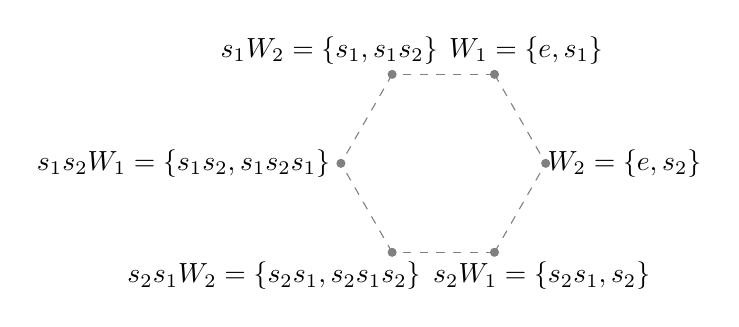
\begin{tikzpicture}
  \def\offX{0.65}
  \def\offY{1.13}
	\draw[dashed,color=gray] (0+\offX,0+\offY) -- (0.65+\offX,-1.13+\offY);% e to s_1
  \draw[dashed,color=gray] (0+\offX,0-\offY) -- (0.65+\offX,-1.13+\offY);% e to s_2
	\draw[dashed,color=gray] (0+\offX,0+\offY) -- (0-\offX,0+\offY);% s_1 to s_1s_2
  \draw[dashed,color=gray] (0+\offX,0-\offY) -- (0-\offX,0-\offY);% s_2 to s_2s_1
  \draw[dashed,color=gray] (0-\offX,0+\offY) -- (-1.3,0);% s_1s_2 to s_1s_2s_1
  \draw[dashed,color=gray] (0-\offX,0-\offY) -- (-1.3,0);% s_2s_1 to s_2s_1s_2

  \draw [fill=gray, color=gray](1.3,0) circle (0.05);
  \draw [fill=gray, color=gray](-1.3,0) circle (0.05);
  \draw [fill=gray, color=gray](0+\offX,0+\offY) circle (0.05);
  \draw [fill=gray, color=gray](0-\offX,0+\offY) circle (0.05);
  \draw [fill=gray, color=gray](0+\offX,0-\offY) circle (0.05);
  \draw [fill=gray, color=gray](0-\offX,0-\offY) circle (0.05); % s_1s_2

  \draw (2.3,0) node {$W_2 = \{e,s_2\}$};
  \draw (-3.3,0) node {$s_1s_2W_1 = \{s_1s_2,s_1s_2s_1\}$};
  \draw (0+\offX + 0.40,0+\offY + 0.30) node {$W_1 = \{e,s_1\}$};
  \draw (0+\offX + 0.60,0-\offY - 0.30) node {$s_2W_1 = \{s_2s_1,s_2\}$};
  \draw (0-\offX - 0.80,0+\offY + 0.30) node {$s_1W_2 = \{s_1,s_1s_2\}$};
  \draw (0-\offX - 1.5,0-\offY - 0.30) node {$s_2s_1W_2 = \{s_2s_1,s_2s_1s_2\}$};
\end{tikzpicture}
\end{center}
\caption{A simplicial complex.}
\label{fig:simplicial}
\end{figure}

\begin{example}
  For the sets $W_1 = W_{s_1} = {e,s_1}$ and $W_2 = W_{s_2} = {e,s_2}$ we have in figure \ref{fig:simplicial} the representation of its simplicial complex. You may notice that the nodes are adjacent if they have an element in common.
\end{example}


\section{Some representation theory}
The purpose of this section is to prove the following theorem :
\begin{theorem}\label{Le theorem W fini si et seulement si on  aun produit scalaire}
	Let $(W,S)$ be a Coxeter system then the Coxeter group $W$ is finite if and only if the symmetric bilinear form, we defined on the associated vector space  $V=<\{\alpha_1,...,\alpha_n\}>$ by :
	\begin{equation}
	\prods{\alpha_i}{\alpha_j}_V\qq=\qq \begin{cases}
	\qq -\cos(\pi/m(s_i,s_j))\q\q&\mbox{if }m(s_i,s_j)<+\infty\\
	\q -1&\mbox{if }m(s_i,s_j)=+\infty
	\end{cases}
	\end{equation}
	is positive definite on $V$.
\end{theorem}
The proof of this theorem is done by using some topology and some representation theory. First of all let us prove that if the symmetric bilinear form is positive definite, then $W$ must be finite.

Let $(W,S)$ be a Coxeter system and let $\pi$ denotes the injective group homomorphism of Theorem \ref{Theorem de l'extension en un morphisme injectif de groupe.}. Since this one defines a group homomorphism :
\begin{equation}
\pi\fctt{W}{\mbox{GL(V)}},
\end{equation}
it is by definition a representation of the Coxeter group $W$ with representation space $V=<\{\alpha_1,...,\alpha_n\}>$. In particular, we can consider the contragredient representation $\pi^*$ of $\pi$ defined as :
\begin{equation}
\pi^*\fct{W}{\mbox{GL}(V^*)}{w}{\sigma(w^{-1})^T},
\end{equation}
where $V^*$ denotes the dual vector space of $V$ and $A^T$ denote the transpose of $A$ for every $A\in \Hom(V,V)$, in other words, for every $f\in V^*$ we have that $A^T(f)=f\circ A$. Since, the representation $\pi$ was faithful, namely since the group automorphism $\pi$ was injective, it is clear that its contragredient representation $\pi^*$ must also be faithful. In particular, this means that $W$ can be seen as a subgroup $\pi^*(W)$ of $\mbox{GL}(V)$. Furthermore, by denoting the natural pairing between $V^*$ and $V$ by $(\cdot,\cdot)$ :
\begin{equation}
(\cdot,\cdot)\fct{V^*\times V}{\R}{(f,v)}{f(v)},
\end{equation}
we see that for every $w\in W$ and for all $f\in V^*,\qq v\in V$ we have that :
\begin{equation}
\begin{split}
(\pi^*(w)f,v)\qq&=\qq \pi^*(w)f(v)\\
&=\qq \pi(w)^Tf(v)\qq\\
&=\qq f\circ\pi(w)(v)\qq\\
&=\qq f(\pi(w)v)\qq\\
&=\qq (f,\pi(w)v).
\end{split}
\end{equation}
Now, let us equip the group $\pi^*(W)$ with a natural topology. Since
\begin{equation}
\pi^*(W)\sub \mbox{GL}(V^*)\sub\Hom(V^*,V^*)\simeq\R^{n^2},
\end{equation}
we see that $\Hom(V^*,V^*)$ can be equipped with the natural topology of balls associated with any finite dimensional real vector space and therefore, we can consider the quotient topology on $\pi^*(W)$ naturally induced on $\pi^*(W)$ by the inclusion map. We have the following Lemma :
\begin{lemma}
	The topology induced on $\pi^*(W)$ by the inclusion map into $\Hom(V^*,V^*)$ is the discrete topology. In other words, every sets of the form $\{g\}$ for some $g\in \pi^*(W)$ defines an open of $\pi^*(W)$.
\end{lemma}
\begin{proof}
	Take any point $f\in V^*$, then, we can consider the map :
	\begin{equation}
	\mbox{ev}_f\fct{\mbox{GL}(V^*)}{V^*}{g}{g(f)}.
	\end{equation}
	This map is continuous for every $f\in V^*$ because it is linear and any linear operator between finite dimensional vector spaces must be continuous for the unique normed topology associated. Furthermore, since the :
	\begin{equation}
	A_{s_i}\qq=\qq \{f\in V^*\qq :\qq (f,\alpha_i)>0\}
	\end{equation}
	defines open subsets of $V^*$ for every $i=1,...,n$, and since every finite intersection of open stays open, the fundamental chamber $C=\bcap{i=1}{n}A_{s_i}$ of $W$ is an open subset of $V^*$. In particular, since the preimage of any open set by a continuous map is by definition an open set, this implies that for every $f\in V^*$ the set :
	\begin{equation}
	Z_f\qq=\qq \{g\in \mbox{GL}(V^*)\qq:\qq g(f)\in C\}\qq=\qq \mbox{ev}_f^{-1}
	\end{equation}
	is an open subset of $\mbox{GL}(V^*)$. In particular, for every element of the fundamental chamber $f \in C\sub V^*$, the set $Z_f$ must defines an open neighbourhood of the identity $\mbox{Id}_{V^*}\fctt{V^*}{V^*}$ since $\mbox{Id}_{V^*}\in Z_f$ and since $Z_f$ defines an open set of $\mbox{GL}(V^*)$. Because of the first point of Theorem \ref{le gros theorem en 3 points qui decrit le comportement de la chambre, du cone de tites,...} and since $C=C_\es$, we know that the only element $w\in W$ such that $\pi(w)(C)\cap C\not=\es$ is $1_W$ because $W_\es=\{1_G\}$ is the set of stabiliser of $C_\es$, we obtain that $\pi(1_G)=\mbox{Id}_{V^*}$ is the only element of $\pi^*(W)$ which is in $Z_f$. In symbols, this means that :
	\begin{equation}
	Z_f\cap \pi^*(W)\qq=\qq \{\mbox{Id}_{V^*}\},
	\end{equation}
	defines an open neighbourhood of $\mbox{Id}_{V^*}$ in $\pi^*(W)$, but, since this groups defines a topological group, as this is a subgroup of the topological group $\mbox{GL}(V^*)$ equipped with the induced topology, we know that the left multiplication by any element $\pi^*(w)\in \pi^*(W)$ :
	\begin{equation}
	\mbox{Mult}_{\pi^*(w)}\fct{\pi^*(W)}{\pi^*(W)}{\pi^*(w')}{\pi^*(w)\pi^*(w')}
	\end{equation}
	defines an homeomorphism. In particular, we see that the set :
	\begin{equation}
	\{\pi^*(w)\}\qq=\qq \mbox{Mult}_{\pi^*(w)}\{\mbox{Id}_{V^*}\},
	\end{equation}
	defines an open neighbourhood of $\pi^*(w)$ and since this holds for every ${\pi^*(w)}\in \pi^*(W)$, the group $\pi^*(W)$ must be discrete.
\end{proof}
This allow us to prove what we announced before :
\begin{theorem}[First implication of Theorem \ref{Le theorem W fini si et seulement si on  aun produit scalaire}]
	If the symmetric bilinear form  $\prods{}{}_V$ defined on $V$ is positive definite, then $W$ must be finite.
\end{theorem}
\begin{proof}
	We suppose that the symmetric bilinear form $\prods{}{}_V$ defined on $V$ is positive definite, therefore, this defines a scalar product on $V$. Now, let us remark that, because of the second point of Proposition \ref{les sigma definisse une isometrie.}, for every $v_1,v_2\in V$ we have that :
	\begin{equation}
	\prods{\pi(w)v_1}{\pi(w)v_2}_V\qq=\qq \prods{v_1}{v_2}_V.
	\end{equation}
	Therefore,  $\pi(W)$ defines a set of isometries for the scalar product $\prods{}{}_V$ on $V$. In particular, this means that $\pi(W)\sub \mathcal{O}(V)$, where $\mathcal{O}(V)$ denotes the the set of all orthonormal transformation of $V$.
	Now, let us remark that the scalar product $\prods{}{}$ induce a scalar product on the dual space $V^*$. Indeed, it suffices to fix an orthonormal basis $\{e_1,...,e_n\}$ of $V$, to consider its dual basis $\{e_1^*,...,e_n^*\}$ which because of Riesz representation Theorem is exactly to the dual basis $\{\prods{e_1}{}_V,...,\prods{e_n}{}_V\}$ and then defines :
	\begin{equation}
	\prods{e_i^*}{e_j^*}_{V^*}\qq:=\qq\prods{e_i}{e_j}_V\qq=\qq \delta_{ij}.
	\end{equation}
	Under this definition and since $\pi(W)\sub \mathcal{O}(V)$ we see that $\pi^*(W)\sub \mathcal{O}(V^*)$ because the transpose of an orthonormal operator is an orthonormal operator in the dual space. Now, let us remark that $\mathcal{O}(V^*)$ is closed in $\Hom(V^*,V^*)\sub \R^{n^2}$. Indeed, since $\prods{}{}_V^*$ is a symmetric bilinear form, it correspond to some symmetric matrix $A$ in a fixed basis $\{e_1^*,...,e_n^*\}$ of $V^*$. Furthermore, under this correspondence, a matrix $B$ correspond to an element of $\mathcal{O}(V^*)$ if and only if it is solution of the equation :
	 \begin{equation}
	 BAB^T\qq=\qq A.
	 \end{equation}
	 This defines a closed condition and therefore $\mathcal{O}(V^*)$ is a closed set in $\Hom(V^*,V^*)\simeq\R^{n^2}$. Remark that we did not use the fact that the bilinear form $\prods{}{}_V$ was positive definite to show that $\mathcal{O}(V^*)$ is a closed set. Furthermore, since every norm on finite dimensional vector space are equivalent and since every matrices of $\mathcal{O}(V^*)$ is bounded for the norm $\norm{\cdot}{\infty}$ defined as $\norm{A}{\infty}=\underset{i,j\in \{1,..,n\}}{\mbox{max}}\qq A_{i,j}$ for every matrix $A\sub \R^{n^2}$, we see that $\mathcal{O}(V^*)$ is bounded in $\Hom(V^*,V^*)$. Therefore, the set $\mathcal{O}(V^*)$ is closed and bounded in the finite dimensional normed vector space $\Hom(V^*,V^*)$, and the Riesz theorem implies that $\mathcal{O}(V^*)$ is a compact set. Furthermore, the previous lemma showed that $\pi^*(W)$ was equipped with the discrete topology. Since it is contained in a compact, the only possibility is that $\pi^*(W)$ is finite, but since $\pi^*$ was injective, this implies that $W$ is finite.
\end{proof}
The second implication of Theorem \ref{Le theorem W fini si et seulement si on  aun produit scalaire} will require some representation theory that we develop just below.

\begin{definition}
	Let $G$ be a finite group and let $\pi \fctt{G}{\mbox{GL(V)}}$ define a representation of $G$ in some real finite dimensional vector space $V$. Then, a bilinear form $\prods{}{}$ defined on $V$ is said to be $G$-invariant if for every $u,v\in V$ and all $g\in G$ we have that :
	\begin{equation}
	\prods{\pi(g)u}{\pi(g)v}\qq=\qq \prods{u}{v}.
	\end{equation}
\end{definition}
The following lemma implies that such a form always exists.
\begin{lemma}\label{existence of a g invariant non degenerate bilinear form on the representaion sapce}
	For every finite group $G$ and every representation $\pi \fctt{G}{\mbox{GL(V)}}$ of $G$ in a real finite dimensional vector space $V$, there exists some $G$-invariant positive definite bilinear form on $V$.
\end{lemma}
\begin{proof}
	The proof is straight forward. Let us consider any basis $\{e_1,...,e_n\}$ of $V$. Form this point, we can define some bilinear non degenerate form on $V$ by setting on the basis :
	\begin{equation}
	\prods{e_i}{e_j}_V\qq=\qq \delta_{ij},
	\end{equation}
	and by extending the bilinear form on $V$ by linearity. Now, let us define for every $u,v\in V$ :
	\begin{equation}
	\prods{u}{v}\qq=\qq \s{g\in G}{}\prods{\pi(g)u}{\pi(g)v}_V.
	\end{equation}
	This defines a $G$-invariant bilinear symmetric form on $V$. The positive definite character follows from the fact that $\prods{u}{u}\geq 0$ with equality if and only if $u=0$ since $\prods{\pi(g)u}{\pi(g)u}_V\geq 0$ and since $\prods{\pi(1_G)u}{\pi(1_G)u}_V=\prods{u}{u}_V\geq 0$ with equality if and only if $u=0$.
\end{proof}
Now, let us make some definitions :
\begin{definition}
	Let $G$ be a finite group and let $\pi \fctt{G}{\mbox{GL(V)}}$ defines a representation of $G$ in some real finite dimensional vector space $V$, we say that $W\sub V$ is a $G$-invariant subspace of $V$ if and only if $\pi(g)W\sub W$ for every $g\in G$.
\end{definition}
Let us remark that $\{0\}$ and $V$ always defines $G$-invariant subspaces of $V$.
\begin{definition}
	Let $G$ be a finite group and let $\pi \fctt{G}{\mbox{GL(V)}}$ define a representation of $G$ in some real finite dimensional vector space $V$, we say that $\pi$ is irreducible if and only if there is no $G$-invariant subspaces of $V$ but the trivial ones $\{0\}$ and $V$.
\end{definition}
\begin{theorem}
	Let $G$ be a finite group and let $\pi \fctt{G}{\mbox{GL(V)}}$ define a representation of $G$ in some real finite dimensional vector space $V$. If $U\sub V$ defines a non-trivial $G$-invariant subspace of $V$, then, there exists some $U'\sub V$ which is also $G$-invariant and such that :
	\begin{equation}
	U\qq \oplus \qq U'\qq=\qq V.
	\end{equation}
\end{theorem}
\begin{proof}
	Let us consider some $G$-invariant bilinear form $\prods{}{}$ on $V$ and let us define :
	\begin{equation}
	U'\qq=\qq U^\perp\qq=\qq\{v\in U\qq :\qq \prods{u}{v}=0\q \forall u\in U\}.
	\end{equation}
	It is not hard to see that :
	\begin{equation}
	U\qq \oplus \qq U'\qq=\qq V.
	\end{equation}
	Furthermore, for every $g\in G$, very $u\in U$ and every $v\in U'=U^\perp$ we have that :
	\begin{equation}
	\prods{u}{\pi(g)v}\qq=\qq \prods{\pi(g^{-1})u}{v}\qq=\qq 0.
	\end{equation}
	The last equality following from the fact that $U$ is $G$-invariant and that $v\in U^\perp$ and we deduce that $U^\perp$ is $G$-invariant.
\end{proof}
\begin{definition}
	Let $G$ be a finite group and let $\pi \fctt{G}{\mbox{GL(V)}}$ define a representation of $G$ in some real finite dimensional vector space $V$. We define the centralizer of $\pi$ as the set :
	\begin{equation}
	Z_G\qq=\qq \{A\in \mbox{GL(V)}\qq :\qq A\pi(g)=\pi(g)A\qq\forall g\in G\}.
	\end{equation}
\end{definition}
Now, let us recall the reciprocate of Schur's Lemma :
\begin{lemma}\label{si le centralisateur n'est fait que d'application scalaire, alors V est irreductible}
	Let $G$ be a finite group and let $\pi \fctt{G}{\mbox{GL(V)}}$ define a representation of $G$ in some real finite dimensional vector space $V$, then, if the centraliser of $\pi$ consists only of scalar operators :
	\begin{equation}
	Z_G(V)\qq=\qq \{c\mbox{Id}_V\qq :\qq c\in \R\backslash\{0\}\},
	\end{equation}
	the representation $\pi$ must be irreducible.
\end{lemma}
\begin{proof}
	Suppose by absurd that $\pi$ is not irreducible, and let $U$ denotes some non trivial $G$-invariant subspace of $V$. Using previous lemma, we know that there exists some other non trivial $G$-invariant subspace $U'$ of $V$ such that $U\oplus U'=V$.
	Now, let us consider the projection :
	\begin{equation}
	P_U\qq\fct{V}{U}{u+u^\perp}{u}.
	\end{equation}
	Since $U$ is a $G$-invariant subspace of $V$, and due to previous lemma the map $P_U$ defines a $G$-morphism between $V$ and $U$. Indeed, for all $g\in G$ and for all $u+u'\in U\oplus U'=V$ we have that :
	\begin{equation}
	P_U(\pi(g)(u+u'))\qq=\qq P_U(\pi(g)u+\pi(g)u')\qq=\qq \pi(g)u,
	\end{equation}
	since from the $G$-invariance of $U$ and $U'$ we have that $\pi(g)u\in U$ and $\pi(g)u'\in U'$. In particular, we conclude that $P_u$ defines a $G$ morphism from $V$ to $V$ since $P_U\pi(g)=\pi(g)P_U$. Using the same argument, the projection on $U'$,  $P_{U'}$ also defines a $G$-morphism from $V$ to $V$. Therefore, $P_U,P_{U'}\in Z_G(V)$. In particular, this means that :
	\begin{equation}
	P_u\qq+\qq 2\qq P_{U'}\qq \in Z_G(V).
	\end{equation}
	Therefore, by hypothesis $P_u\qq+\qq 2\qq P_{U'}\qq=\qq c\mbox{Id}_V$ for some $c\in \R\backslash\{0\}$. This is a contradiction with the fact that $U$ and $U'$ are non trivial subspaces and that $P_U$ and $P_{U'}$ defines scalar operators on $V$ since they also defines element of $Z_G(V)$.
\end{proof}
Under the same hypothesis, it is possible to show that there exists up to multiplication by a scalar, a unique non degenerate $G$-invariant bilinear form on $V$.
\begin{lemma}
		Let $G$ be a finite group and let $\pi \fctt{G}{\mbox{GL(V)}}$ define a representation of $G$ in some real finite dimensional vector space $V$, then, if the centraliser of $\pi$ consists only of scalar operators :
		\begin{equation}
		Z_G(V)\qq=\qq \{c\mbox{Id}_V\qq :\qq c\in \R\backslash\{0\}\},
		\end{equation}
		then, there exists up to multiplication by a scalar, a unique non degenerate $G$-invariant bilinear form on $V$.
\end{lemma}
\begin{proof}
	The existence of such a bilinear form is guaranteed by Lemma \ref{existence of a g invariant non degenerate bilinear form on the representaion sapce}. It last to show the unicity up to multiplication by a scalar. Following this purpose, let us consider $\prods{}{}_1$ and $\prods{}{}_2$. Let us fix a basis $\{u_1,...,u_n\}$ of $V$. Now, let us consider a basis $\{v_1,...,v_n\}$ of $V$ which is dual to the basis $\{u_1,...,u_n\}$ with respect to the scalar product $\prods{}{}_1$, which means that $\prods{u_i}{v_j}_1=\delta_{ij}$. Similarly, let us consider basis $\{w_1,...,w_n\}$ of $V$ which is dual to the basis $\{u_1,...,u_n\}$ with respect to the scalar product $\prods{}{}_2$, which means that $\prods{u_i}{w_j}_2=\delta_{ij}$. Let us define a linear application $\varphi\fctt{V}{V}$, by the relation $\varphi(v_i)=w_i$. Then, it is clear that $\varphi\in \mbox{GL}(V)$. Furthermore, for every $i,j\in \{1,...n\}$ and for all $g\in G$ we have that :
	\begin{equation}
	\prods{u_i}{\varphi(v_j)}_2\qq=\qq \prods{u_i}{w_j}_2\qq=\qq \delta_{ij}\qq=\qq\prods{u_i}{v_j}_1
	\end{equation}
	In particular, this implies that for every $u,v\in V$ and for all $g\in G$, we have that :
	\begin{equation}
	\begin{split}
	\prods{u}{\pi(g)\varphi(v)}_2\qq&=\qq \prods{\pi(g^{-1})u}{\varphi(v)}_2\qq\\
	&= \qq \prods{\pi(g^{-1})u}{v}_1\\
	&=\qq  \prods{u}{\pi(g)v}_1\\
	&=\qq  \prods{u}{\varphi(\pi(g)v)}_2.
	\end{split}
	\end{equation}
	Therefore, by non degeneracy of the scalar product $\prods{}{}_2$, we obtain that $\pi(g)\varphi(v)=\varphi(\pi(g)v)$ for every $v\in V$ and for all $g\in G$. Therefore, this implies that $\varphi\in Z_G(V)$, and by hypothesis, there exists some $c\in \R\backslash\{0\}$ such that $\varphi=c\mbox{Id}_V$, which means that :
	\begin{equation}
	\prods{u}{v}_1\qq=\qq\prods{u}{\varphi(v)}_2\qq=\qq c\prods{u}{v}_2.
	\end{equation}
	This proves as wanted that $\prods{}{}_1=c\prods{}{}_2$ for some $c\in \R\backslash\{0\}$.
\end{proof}
\begin{proposition}\label{la seule form G invariante non nul est positve si jamais on a un centralizer scalaire}
	Let $G$ be a finite group and let $\pi \fctt{G}{\mbox{GL(V)}}$ define a representation of $G$ in some real finite dimensional vector space $V$, then, if the centraliser of $\pi$ consists only of scalar operators :
	\begin{equation}
	Z_G(V)\qq=\qq \{c\mbox{Id}_V\qq :\qq c\in \R\backslash\{0\}\},
	\end{equation}
	the only non zero $G$-invariant symmetric bilinear form up to multiplication by a scalar is the positive definite one.
\end{proposition}
\begin{proof}
	Let $\prods{}{}$ be a non zero $G$-invariant symmetric bilinear from. Then the space :
	\begin{equation}
	V^\perp\qq=\qq \{v\in V\qq :\qq \prods{v}{w}=0\qq\forall w\in V\}
	\end{equation}
	is a $G$-invariant subspace of $V$. But due to Lemma \ref{si le centralisateur n'est fait que d'application scalaire, alors V est irreductible}, $\pi$ is irreducible and therefore, since $\prods{}{}$ is non zero, this implies that $V^\perp=\{0\}$. We conclude that $\prods{}{}$ is non degenerate and therefore, applying the previous Lemma, we conclude that there must exists a constant $c$ such that our bilinear form $\prods{}{}$ is multiple of the positive definite one given by Lemma \ref{existence of a g invariant non degenerate bilinear form on the representaion sapce}.
\end{proof}

Now, let us come back to the study of Coxeter groups.
Having this last proposition in mind, we just need to show that the centraliser of $W$ given by our representation $\pi \fctt{W}{\mbox{GL}(V)}$ is exactly $\{c\mbox{Id}_V\qq:\qq c\in \R\backslash\{0\}\}$ to prove the second implication of Theorem \ref{Le theorem W fini si et seulement si on  aun produit scalaire}. This require just a little bit of work.

\begin{definition}
	A Coxeter system $(W,S)$ is said to be irreducible if the corresponding Coxeter graph is connected.
\end{definition}
\begin{lemma}
	If $(W,S)$ is an irreducible Coxeter system, then the centraliser of the representation $\pi$ consists of scalar operators :
	\begin{equation}
	Z_W(V)\qq=\qq\{c\mbox{Id}_V\qq:\qq c\in \backslash\{0\}\}
	\end{equation}
\end{lemma}
\begin{proof}
	Let $A$ be an element of the centralizer of $\pi\fct{W}{\mbox{GL}(V)}{s_i}{\sigma_{\alpha_i}}$, namely $A\in Z_W(V)$. Then, by definition $A$ commutes with the application $\sigma_\alpha$ where $\alpha\in \Delta=\{\alpha_1,...,\alpha_n\}$ is a simple root of $V$. Therefore, we obtain that :
	\begin{equation}
	\sigma_\alpha A\alpha\qq=\qq A\sigma_\alpha\alpha\qq=\qq A(-\alpha) \qq=\qq -A(\alpha).
	\end{equation}
	In particular, this implies that $A\alpha=c_\alpha\alpha$ for some $c_\alpha\in \R\backslash\{0\}$ since $\sigma_\alpha(\phi^+\backslash\{\alpha\})=\phi^+$ and since $A\in \mbox{GL}(V)$. Now, let $\beta\in\Delta$ be any simple root of $V$, then, we obtain that :
	\begin{equation*}
	A\sigma_\alpha\beta\qq=\qq \sigma_\alpha A\beta
	\end{equation*}
	\begin{equation*}
	\iff \q A\qq \big(\beta\qq-\qq 2\frac{\prods{\alpha}{\beta}}{\prods{\alpha}{\alpha}}\alpha\big)\qq=\qq A(\beta)\qq -\qq 2\frac{\prods{A(\beta)}{\alpha}}{\prods{\alpha}{\alpha}}\alpha
	\end{equation*}
	\begin{equation*}
	\iff \q A(\beta)\qq-\qq 2\frac{\prods{\alpha}{\beta}}{\prods{\alpha}{\alpha}}A(\alpha)\qq=\qq A(\beta)\qq -\qq 2\frac{\prods{c_\beta\beta}{\alpha}}{\prods{\alpha}{\alpha}}\alpha
	\end{equation*}
	\begin{equation*}
	c_\alpha\prods{\alpha}{\beta}\qq\alpha \qq =\qq c_\beta\qq \prods{\beta}{\alpha}\qq \alpha
	\end{equation*}
	From this last equality, we identify two cases. Either $c_\alpha=c_\beta$ or $\prods{\alpha}{\beta}=0$ which means that $\sigma_\alpha$ and $\sigma_\beta$ commutes. Since the Coxeter graph associated to $W$ is connected, we see that for any two simple roots $\alpha,\beta$ there exists a path of non commuting simple roots $\alpha=\alpha'_1,...,\alpha'_k=\beta$ and we therefore obtain that $c_\alpha=c_{\alpha'_1}=c_{\alpha'_2}=...=c_{\alpha'_k}=c_\beta$, which proves that $c_\alpha=c_\beta$ for any two simple roots $\alpha,\beta\in \Delta$. In particular, this implies that $A=c\mbox{Id}_V$ for some $c\not=0$.
\end{proof}

This implies the second implication of Theorem \ref{Le theorem W fini si et seulement si on  aun produit scalaire} :
\begin{theorem}[Second implication of Theorem \ref{Le theorem W fini si et seulement si on  aun produit scalaire}]
	If $W$ is finite, the symmetric bilinear form  $\prods{}{}_V$ defined on $V$ must be positive definite.
\end{theorem}
\begin{proof}
	As we already remarked before, because of Proposition \ref{la seule form G invariante non nul est positve si jamais on a un centralizer scalaire} it suffices to show that :
	\begin{equation}
	Z_W(V)\qq=\qq\{c\mbox{Id}_V\qq:\qq c\in \R\backslash\{0\}\}
	\end{equation}
	for the Theorem to handle. First of all, let us remark that if $(W,S)$ is a coxeter system such that its Coxeter graph $\Gamma$ can be written as a disjoint union of two other non empty graphs $\Gamma=\Gamma_1\sqcup \Gamma_2$ then, both $\Gamma_1$ and $\Gamma_2$ are the Coxeter graphs of some parabolic subgroup $W_{I_1}$ and $W_{I_2}$ of $W$ such that $S=I_1\sqcup I_2$ and therefore,
	\begin{equation}
	W\qq\simeq\qq W_{I_1}\qq \times \qq W_{I_2}
	\end{equation}
	Since the relation between elements of  $W_{I_1}$ and $W_{I_2}$ are consists only of the commutation of any two elements. In particular, this implies that for any $i\in I_1$ and any $j\in I_2$, $m(s_i,s_j)=2$ in particular, this implies that $\prods{\alpha_i}{\alpha_j}=-\cos(\pi/m(s_i,s_j))=0$ and we see that the matrix of $\prods{}{}$ in the basis $\Delta=\{\alpha_1,...,\alpha_n\}$ is of the form :
	\begin{equation}
	\begin{bmatrix}
	A_{I_1} & 0\\
	0 & A_{I_2}
	\end{bmatrix}
	\end{equation}
	where $A_{I_1}$and $A_{I_2}$ denotes the matrix of the bilinear form associated to the new Coxeter groups $W_{I_1}$ and $W_{I_2}$ which coincide with the restriction og $\prods{}{}$ to the subspaces of $V$ generated by $\{\alpha_i:i\in I_1\}$ and $\{\alpha_i:i\in I_2\}$ respectively. In particular, by iteration, we can restrict our attention to the connected component of the Coxeter graph $\Gamma$ which therefore correspond to an irreducible parabolic subgroup $W_I$ of $W$. Furthermore, by the previous Lemma, and what we remarked before, the restriction of $\prods{}{}$ on the parabolic subgroup $W_I$ is positive definite. This implies that $\prods{}{}$ is positive definite and the Theorem is proved.
\end{proof}

\section{Classification of the Coxeter groups}

Let $(W,S)$ be a Coxeter system and $(m_{ij})$ the associated Coxeter matrix. As discussed above, if $V$ is a real vector space with basis $\{\alpha_1, \ldots , \alpha_n\}$, we can define a symmetric bilinear form as
\begin{equation}
\langle \alpha_i , \alpha_j \rangle = \left \{
\begin{array}{c @{} c}
    &- \cos \left(\frac{\pi}{m_{ij}} \right) \quad \text{if } m_{ij} < + \infty \\
    &-1 \quad ~~~~~~~~~~~~~\text{if } m_{ij} = + \infty \\
\end{array}
\right.
\end{equation} We proved above that $W$ is finite if and only if $\langle ., . \rangle$ is positive definite.

\begin{definition}
$W$ is irreducible if its Coxeter graph is connected.
\end{definition}

This definition can be understood from the following observation: if $\Gamma = \Gamma_1 \sqcup \Gamma_2$, then $W_\Gamma = W_{\Gamma_1} \times W_{\Gamma_2}$.

Let us now introduce some basic notations. Take $\{ e_1, \ldots, e_n \}$ be a basis of a vector space $V$. Take $v = \sum_i x_i e_i$ and $w =  \sum_i y_i e_i$ in $V$. Writing $g_{ij} = \langle e_i , e_j \rangle$, we have
\begin{equation}
\begin{split}
\langle v, w \rangle &= \sum_i \sum_j x_i y_j \langle e_i, e_j \rangle \\
&= \sum_i \sum_j x_i y_j g_{ij} \\
&= x^T g y
\end{split}
\end{equation} where, in the last equality, we used matrix notation.

\begin{lemma} [Sylvester]
$\langle ., . \rangle$ is positive definite if and only if all the principal minors of $g$ are positive.
\end{lemma}
\begin{proof}
The condition is necessary. In fact, taking $v = (v_1, \ldots , v_r , 0, \ldots , 0)$, we have $\langle v, v \rangle = v^T g v$.

The condition is also sufficient. In order to show it, let us proceed by induction on the size of $g$. If $g$ is not positive definite, there must be $2$ negative eigenvalues since the determinant is positive. Let $x \neq 0 \neq y$ be $2$ orthogonal eigenvectors associated to these eigenvalues. Let $\alpha, \beta \in \mathbb{R}$ such that $(\alpha, \beta) \neq (0, 0)$. We write
\begin{equation}
v := \alpha x + \beta y = (*, *, \ldots , * 0 ) \neq 0
\end{equation}   We have
\begin{equation}
v^T g v = \alpha^2 x^T g x + \beta^2 y^T g y \le 0
\end{equation} This implies that that the determinant is non-positive.
\end{proof}

\begin{theorem}
The irreducible finite Coxeter groups are given in figure \ref{Classification}.
\begin{figure}[h!]
\centering
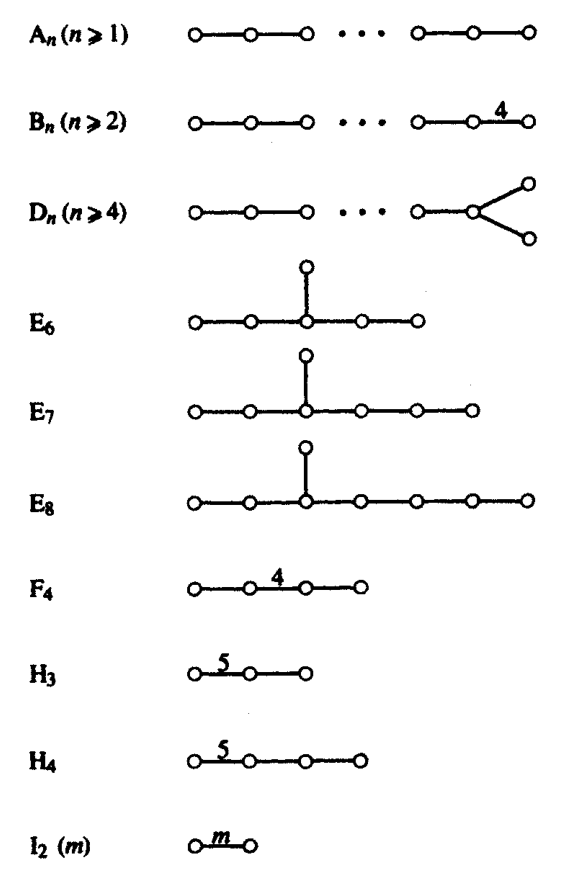
\includegraphics[scale=0.6]{Classification.png}
%\caption{The }
\label{Classification}
\caption{}
\end{figure}
\label{classification thm}
\end{theorem}

\begin{remark}
Define the matrix $A_\Gamma$ by $[A_\Gamma]_{ij} = 2 \langle \alpha_i , \alpha_j \rangle$ and set $d(\Gamma) = \det (A_\Gamma ) $. We make the following observations:
\begin{itemize}
\item Removing one node in a diagram is equivalent to remove the associated line and column.
\item If $\Gamma = \Gamma_1 \sqcup \Gamma_2$, then $d(\Gamma ) = d (\Gamma_1). d(\Gamma_2)$.
\end{itemize}
\end{remark}

\begin{lemma}
Let $\Gamma$, $\Gamma '$ and $\Gamma ''$ be as in figure \ref{cours9fig1}.

\begin{figure}[h!]
\centering
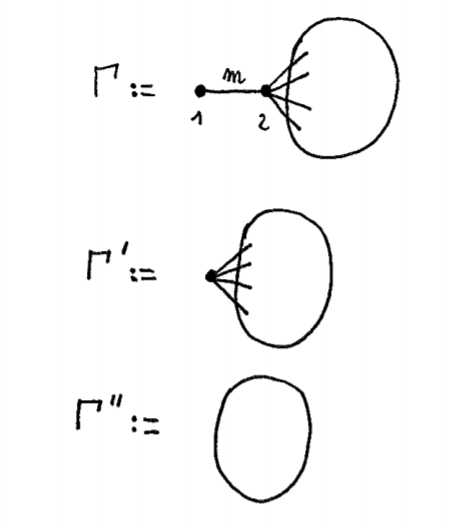
\includegraphics[scale=0.6]{cours9fig1.png}
\caption{}
\label{cours9fig1}
\end{figure}

Then $d(\Gamma) = 2 d(\Gamma ') - 4 \cos^2 \left(\frac{\pi}{m} \right) d (\Gamma '')$.
\end{lemma}

\begin{proof}
Consider
\begin{equation}
A = \begin{pmatrix}
2 &-\cos \left(\frac{\pi}{m} \right) &0 &\cdots \\
-\cos \left(\frac{\pi}{m} \right) &2 &\cdots & \\
0 &\vdots & 2 &\cdots \\
\vdots &  & \vdots
\end{pmatrix}
\end{equation} We have
\begin{equation}
d (\Gamma ) =2 d(\Gamma ') - (-2) \cos \left(\frac{\pi}{m} \right) (-2) \cos \left(\frac{\pi}{m} \right)  d (\Gamma '')
\end{equation}
\end{proof}

We now compute $d(\Gamma)$ for all the cases in the classification \ref{classification thm}, using the previous lemma.

\begin{itemize}
\item For the case $A_n$, we have
\begin{equation}
d(A_n) = d(A_{n-1} ) - 4 \cos^2 \left(\frac{\pi}{3} \right) d(A_{n-2}) = n+1
\end{equation} where, to obtain the last equality, we used
\begin{equation}
d(\circ) =2 \quad \text{and} \quad d(\circ-\circ) = \det \begin{pmatrix}
2 &-1 \\
-1 &2
\end{pmatrix} = 3
\end{equation}
\item For $B_n$, we have
\begin{equation}
d(B_n) = 2 d(B_{n-1} ) - d (B_{n-2})
\end{equation} for $n\ge 4$,
\begin{equation}
d(B_3) = 2 d (B_2) - d \circ) = 4-2 = 2
\end{equation} and
\begin{equation}
d(B_2) = \det \begin{pmatrix}
2 &-2 \cos \left(\frac{\pi}{4} \right) \\
-2 \cos \left( \frac{\pi}{4} \right) & 2
\end{pmatrix} = 4 - 4 \cos^2 \left( \frac{\pi}{4} \right) = 2
\end{equation} Therefore, $d(B_n) = 2$.
\item For $D_n$, we have
\begin{equation}
d (D_n) = 2 d(D_{n-1}) - d (D_{n-2})
\end{equation} Furthermore,
\begin{equation}
\begin{split}
d( {}^\circ_\circ > \circ - \circ ) &= 2 d(  {}^\circ_\circ > ) - d ( {}^\circ_\circ) \\
&= 2 d(A_3) - d (A_1)^2 \\
&= 2 . 4 - 2^2 \\
&= 4
\end{split}
\end{equation} and
\begin{equation}
\begin{split}
d(\circ - \circ - \circ < ^\circ_\circ ) &= 2 d (\circ - \circ < ^\circ_\circ ) - d (\circ < ^\circ_\circ) \\
&= 2 .4 - 4 \\
&= 4
\end{split}
\end{equation} We deduce that $d(D_n) = 4$.
\item We proceed in the same way for the other elements the list \ref{classification thm}. We get $d(E_6) = 3$, $d(E_7) = 2$, $d(E_8) = 1$, $d(F_4) = 1$, $d(H_3) = 3 - \sqrt{5} > 0$, $d(H_4) = \frac{7 - 3 \sqrt{5}}{2} > 0$ and $d(I_2 (m) ) = 4 \sin^2 \left( \frac{\pi}{m} \right) > 0$, for $m \ge 3$ ($m= 2$ is disconnected).

\end{itemize}

Now, we have to show that there are no other diagrams. In order to do that, le us make some observations.
\begin{itemize}
\item We cannot have diagrams of the type given in figure \ref{cours9fig2}, because there are no relations between these generators. They generate an infinite group.

\begin{figure}[h!]
\centering
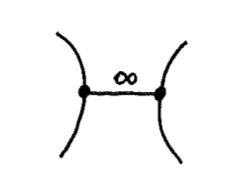
\includegraphics[scale=0.6]{cours9fig2.png}
\caption{}
\label{cours9fig2}
\end{figure}

\item We cannot have circuits, i.e. diagrams of the type of figure \ref{cours9fig3}


\begin{figure}[h!]
\centering
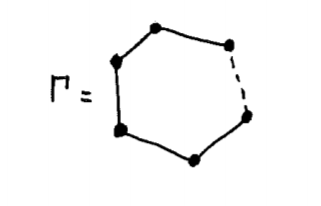
\includegraphics[scale=0.6]{cours9fig3.png}
\caption{}
\label{cours9fig3}
\end{figure}

In fact,
\begin{equation}
A_\Gamma = \begin{pmatrix}
2 &* &0 &\cdots &0 &* \\
* &2 &* &0 &\cdots &0 \\
0 &* &2 &* &0 &\cdots \\
\vdots & & &\ddots & & \\
0 & & & & &* \\
* &0 &\cdots &0 &* &2
\end{pmatrix}
\end{equation} where
\begin{equation}
\begin{split}
* &= - 2 \cos \left( \frac{\pi}{m} \right) \quad (m\ge 3 ) \\
&\le - 2 \cos \left( \frac{\pi}{3} \right) \\
&-1
\end{split}
\end{equation} Therefore,
\begin{equation}
\begin{pmatrix}
1 &\cdots &1
\end{pmatrix} A_\Gamma \begin{pmatrix}
1 \\
\vdots \\
1
\end{pmatrix} = 2n + \sum_{\sharp(*) = 2n} (*) \le 2n - 2n = 0
\label{strategy}
\end{equation} and we conclude that $A_\Gamma$ cannot be positive definite.

\item If $\Gamma$ has at most one edge $>3$. In fact, consider a diagram of the type of figure \ref{cours9fig4}.

\begin{figure}[h!]
\centering
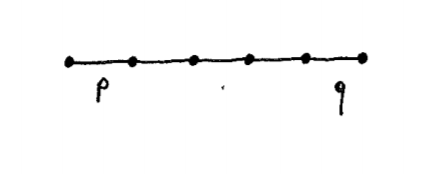
\includegraphics[scale=0.6]{cours9fig4.png}
\caption{}
\label{cours9fig4}
\end{figure}

\begin{equation}
A_\Gamma = \begin{pmatrix}
2 &-2 \cos \left(\frac{\pi}{p}\right) & & & &\\
-2 \cos \left(\frac{\pi}{p}\right) &2 &-1  & & &\\
 &-1 &2 &-1 & &\\
 & &\ddots &\ddots &\ddots & \\
 & & & & & \\
 & & & & &-2\cos\left(\frac{\pi}{p} \right) \\
 & & & &-2 \cos\left(\frac{\pi}{q} \right) &2
\end{pmatrix}
\end{equation} We have
\begin{equation}
\begin{split}
d(A_\Gamma ) &= 2 d(B_{n-1} ) - 4 \cos^2 \left( \frac{\pi}{q} \right) d(B_{n-2} ) \\
&= 4 - 8 \cos^2 \left( \frac{\pi}{q} \right) \\
&\le 0
\end{split}
\end{equation} for $q \ge 4$. The case $q\le 4$ can be done using the same strategy as in \eqref{strategy} and is let as an exercise.

\item If $\Gamma$ has one edge $> 3$, then $\Gamma$ is a straight line. Consider a diagram of the type of figure \ref{cours9fig5}.

\begin{figure}[h!]
\centering
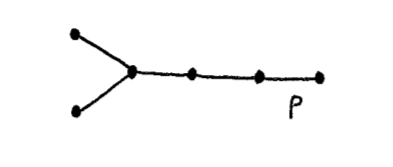
\includegraphics[scale=0.6]{cours9fig5.png}
\caption{}
\label{cours9fig5}
\end{figure}

\begin{equation}
\begin{split}
d(\Gamma ) &= 2 d(\Gamma_{n-1}) - 4 \cos^2 \left( \frac{\pi}{p} \right) d (D_{n-2}) \\
&= 8 - 16 \cos^2 \left( \frac{\pi}{p} \right) \le 0 \\
&\le 0
\end{split}
\end{equation}

\item $\Gamma$ has at most one branching point. In fact consider a diagram of the type of figure \ref{cours9fig6}.

\begin{figure}[h!]
\centering
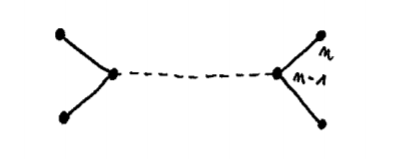
\includegraphics[scale=0.6]{cours9fig6.png}
\caption{}
\label{cours9fig6}
\end{figure}

We have
\begin{equation}
d(\Gamma) = 2 d(\D_{n-1})) - d (D_{n-3} \cup A_1 ) = 8 - 2.4 = 0
\end{equation}

\item $\Gamma$ has no branching point with $4$ or more branches. In fact,
\begin{equation}
\begin{split}
d(>\circ < ) &= 2 d (>\circ - ) - d ({}_\circ^\circ \circ) \\
&= 2 . 4 - 2^3 \\
&=0
\end{split}
\end{equation}

\item It is let as an exercise to show the relations in figure \ref{cours9fig7}.

\begin{figure}[h!]
\centering
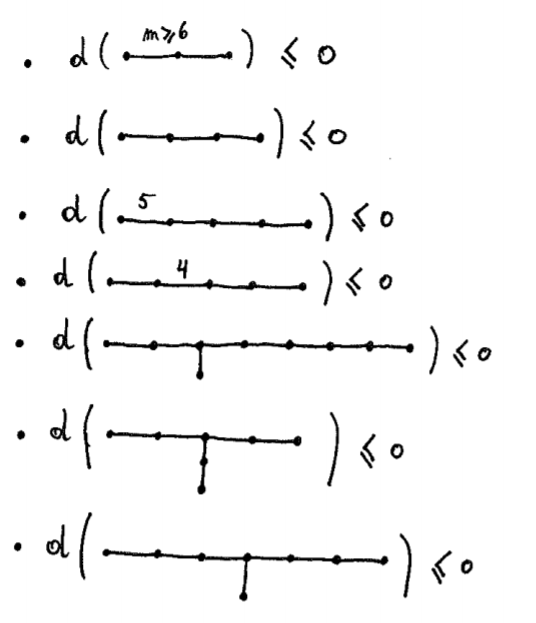
\includegraphics[scale=0.6]{cours9fig7.png}
\caption{}
\label{cours9fig7}
\end{figure}

Therefore, we conclude that no other diagrams than those identified in theorem \ref{classification thm} are valid.

\end{itemize}


\backmatter%%%%%%%%%%%%%%%%%%%%%%%%%%%%%%%%%%%%%%%%%%%%%%%%%%%%%%%
%%%%%%%%%%%%%%%%%%%%%%%% referenc.tex %%%%%%%%%%%%%%%%%%%%%%%%%%%%%%
% sample references
% "computer science"
%
% Use this file as a template for your own input.
%
%%%%%%%%%%%%%%%%%%%%%%%% Springer-Verlag %%%%%%%%%%%%%%%%%%%%%%%%%%

%
% BibTeX users please use
\bibliographystyle{alpha}
\bibliography{main}
%

\printindex

%%%%%%%%%%%%%%%%%%%%%%%%%%%%%%%%%%%%%%%%%%%%%%%%%%%%%%%%%%%%%%%%%%%%%%

\end{document}
